\section{Statistical Framework} \label{sec:stat_fra}
This section introduces a statistical framework that describes the relationship between the design and sample on one side, and the variable of interest on the other sides. The following concepts borrow to  the general statistical framework by  \cite{dbb1}. The definitions and most properties we provide apply in this framework. We also provide a case study example throughout the paper to illustrate the general definitions and properties. Some results presented here only apply to the specific statistical framework used for the example.

\subsection{General notation}

In this paper, all random variables are defined on a probability space $(\Omega,\mathscr{A},P)$. The expected value and variance / covariance operators are defined with respect to the probability measure $P$. 
For two sets $E$ and $F$, $(E\to F)$ or $F^E$ designate the set of the functions from $E$ to $F$.
The notation ``$g:E\to F,x\mapsto g(x)$" means: let $g$ be a mapping from set $E$ to set $F$ that associates $g(x)$ to $x$. For $f:E\to (F\to G)$, $g:E\to F$, $h:E\to (H\to F)$,  the notation $f[g]$ designates the function :  $f[g]:E\to G$, such that $f[g](x)=(f(x))(g(x))$, and the notation 
$f[h]$ designates the function :  $f[h]:E\to (H\to G)$, such that $f[h](x)=(f(x)\circ h(x))$.


For a set $E$, $\bar{E}$ designates the set $\{\mathbf{0}\}\cup\bigcup_{n\in\mathbb{N},n\geq 1} E^{\{1,\ldots,n\}}$, where $\{\mathbf{0}\}=E^\emptyset$ corresponds to the set containing the application $\mathbf{0}$ with empty domain. The application $\mathbf{0}$ can be interpreted as the empty sample that matches no draw to the population of interest. 
Let denote by $\size $ the application that maps an application to the cardinality of its domain: $\bar{E}\to\mathbb{N}$, $\mathbf{e}\mapsto n$ if $\position\in E^{\{1,\ldots,n\}}$, $0$ if $\position=\mathbf{0}$. For an application $\position\in\bar{E}$, a set $\Sampleindex$, $\position_\Sampleindex$ is the application:
$\position_\Sampleindex:\Sampleindex\cap\mathrm{domain}(\position)\to E:\ell\mapsto\position(\ell)$, in the case of a random application $\Sample:\Omega\to\toPop$ and a random set :$\Sampleindex\to(\mathscr{P}(\mathbb{N})$ ($\mathscr{P}(\mathbb{N})$ is the set of all subsets of $\mathbb{N}$), then $\Sample_\Sampleindex$ is the random application: $\Omega\to\toPop, 
\omega\mapsto 
\Sample_\Sampleindex(\omega):(\Sampleindex(\omega)\cap\mathrm{domain}(\Sample(\omega))\to \Pop),
\ell\mapsto (\Sample(\omega))(\ell)$.
For a measure $\eta$ of $E$, a non random finite set $\Sampleindex$, $\eta^{\otimes\Sampleindex}$ is the measure such that for any collection $(\subsetA_\ell)_{\ell\in\Sampleindex}$ of subsets of $E$  :
$\eta^{\otimes\Sampleindex}\left(\bigcap_{\ell\in\mathbb{L}}\{\position\in E^\Sampleindex:\position(\ell)\in\subsetA_\ell\}\right)=\prod_{\ell\in\Sampleindex}\eta(\subsetA_\ell)$, and
$\eta^{\otimes\emptyset}(\{\mathbf{0}\})=1$, 
then define the measure $\bar{\eta}$ on $\bar{E}$: $\bar{\eta}=\eta^{\otimes\emptyset}+\sum_{\samplesize\in\mathbb{N},\samplesize\geq 0}\eta^{\otimes\{1,\ldots,\samplesize\}}$.


We apply the following rule: Random variables are capital Roman letters, whereas Random variable realisations are bold corresponding lowercase roman letter. By convention, any sum over an empty set is 0 and any product over an empty set is 1. The notation $\density_{V\mid W}$ denotes the density of $V$ conditional on $W$ with respect to a dominating measure on the domain of $V$.

\subsection{Spatial process}
We consider a space $\Pop$, that is a compact %(non necessarily convex) 
subset of a finite dimensional real vector space $\mathbb{R}^d$, with its associated Borel sigma-field, and a random process $\Signal$ defined on $\Pop$ with value in another finite dimension real vector space $\SignalSpace$, e.g. $Y:\Omega\to(\Pop\to\SignalSpace)$. %{\color{red} Compacity is required  because blablabla.}
  For example, for a random variable $\Sample:\Omega\to\Pop^{\{1,2\}}$ and a random variable
$\Signal:\Omega\to(\Pop\to\SignalSpace)$, 
$\Signal[\Sample]$ is the random variable: $\Signal[\Sample]:\Omega\to(\{1,2\}\to\SignalSpace)$, $\omega\mapsto(\Signal(\omega))(\Sample(\omega)):\ell\to(\Signal(\omega))(\Sample(\omega)(\ell)$. Examples and illustrations will be given for the particular case where $\Pop=[0,1]^2$.
%Given data $(\position(1),\signal_{1}),...,(\position_{n},\signal_{n})$, in order to perform inference for some target, we postulate a model, which we assume holds for the entire population. In particular, we are interested in model parameters, in other words we focus on \emph{analytic inference}. The choice of the model is not an easy task. It should reflect the structure of the population and should capture the important features useful for inference purpose. An entire branch of literature is dedicated to this task, i.e. \emph{model selection}, but the focus of this paper does not lie in that. 
%For our work we assume that the model describing the variable of interest is given by
%\begin{equation} \label{eq:model}
%\Signal\left[\position\right]=S\left[\position\right]+\epsilon\left[\position\right]
%\end{equation}
%{\color{red} S is for $\Sample$ (sample)}
%where $S\left(\position\right)$ is a zero mean stationary stochastic process in $\mathbb{R}^d$ and is independent from the $\epsilon\left(\position\right)$, which has normal distribution with mean 0 and variance $\sigma_{\epsilon}$. The model in \eqref{eq:model} is quite general and embraces many variations under its umbrella. It is wide known in the field of geostatistics, where the term \emph{kriging} is in vogue. In fact, according to different assumptions about $S(\position)$, we end up with different models, which are usually referred with terms as ordinary kriging, simple kriging, universal kriging and so on. In order to perform inference about the model parameters, we need to introduce some assumptions.
Let $\dominantY$ denote a sigma-finite measure on the set $\SignalSpace$  and let $\dominantU$ denote a probability measure on  $\Pop$.
The {\em $\dominantU$-averaged theoretical semivariogram} is defined as the function: 
\begin{equation}\Semivariogram:\mathbb{R}^d\to[0,+\infty),h\mapsto\frac12\int_{\Pop^{\{1,2\}}} \Var\left[\Signal[\position(2)]-\Signal[\position(1)]\right] \derive(\dominantU^{\otimes \{1,2\}})^{X\mid X[2]-X[1]=h}(\position),\label{eq:averagesemivariogram}\end{equation} 
where $(X)$ is the identity of $\Pop^{\{1,2\}}$, and the {\em $\dominantU$-averaged theoretical covariogram} is the function  $\nu^{X_2-X_1}-a.s(h)$-defined:
\begin{equation}\Covariogram:\mathbb{R}^d\to\mathbb{R}, h\mapsto\int_{\Pop^{\{1,2\}}} \Cov\left[\Signal[\position(1)],\Signal[\position(2)]\right] \derive(\dominantU^{\otimes \{1,2\}})^{X\mid X[2]-X[1]=h}(\position).\label{eq:averagecovariogram}\end{equation} The covariogram and semivariogram satisfy the relationship: $\forall h\in\mathbb{R}^d, \Semivariogram(h)=\Covariogram(0)-\Covariogram(h)$.

%The functions $\Covariogram$ and $\Semivariogram$ satisfy the relationship:
% $$\Covariogram(h)=\Covariogram(0)-\Semivariogram(h)$$.
\begin{definition}[Intrinsic stationarity and Second order stationarity, \protect{\citep[p.~53]{cressie2015statistics}}]
A process is {\em intrinsic stationary} when the following conditions are satisfied :  $\forall \position\in\Pop^{\{1,2\}}$,
\begin{eqnarray}
    \mathrm{E}\left[\Signal\left[\position(2)\right]-\Signal\left[\position(1)\right]\right]&=&0\\
    \frac12~\Var\left[\Signal\left[\position(2)\right]-\Signal\left[\position(1)\right]\right]&=&\Semivariogram(\position(2)-\position(1))\label{eq:semivariogram}
\end{eqnarray}
A process is {\em second order stationary} when the following are satisfied:
\begin{equation}
\exists\mu\in\mathbb{R},~    \forall\position\in \Pop,~~ E\left[\Signal\left[\position\right]\right]=\mu
\end{equation}
\begin{equation} \label{eq:covariogram}
    \forall~\position\in \Pop^{\{1,2\}}, ~\Cov\left[\Signal\left[\position(1)\right],\Signal\left[\position(2)\right]\right]=C\left(\position(1)-\position(2)\right)
\end{equation}
\end{definition}
%The function $\Covariogram\left(\cdot\right)$ in \eqref{eq:covariogram} is called \emph{covariogram}, or \emph{stationary covariance function}. 
In the case of a first order stationary process, the variance operator $\Var[.]$ can equivalently be replaced by the square expected value operator $\mathrm{E}[(.)^2]$ in equation \eqref{eq:averagesemivariogram}.
In the case of a second order stationary process, equations \eqref{eq:averagecovariogram} and \eqref{eq:averagesemivariogram} correspond to the definition of the theoretical covariogram and semivariogram as found in \citet[p.~53 and p.~58]{cressie2015statistics}.
The random process is isotropic if in addition to being second order stationary, the covariogram function $h\mapsto \Covariogram(h)$ only depends on $h$ via $h\mapsto\|h\|$.

%{\color{red} Let us call $\paramnuisance_2$ the parameters for the Semivariogram or $c$ the parameters for the Covariance.
%A plot of the 4 variograms would be neat there. Throughout the paper, $c_0$ should be replaced by $\sigma$}

Common model assumptions on the process $\Signal$ consist in assuming second order stationarity and isotropy. The covariance structure of the signal is then fully characterized by $\Covariogram(0)$ and $\Semivariogram(h), h\neq 0$. 
%We give the  covariogram formal expression for a list of covariogram models. 
For the simulations and illustrations in this paper, a Gaussian covariogram of the form
\begin{equation}\label{def:gaussiancovariogram}\Covariogram(h)=\parampop_1\exp\left(-\|h\|^2/\parampop_2^2\right)\end{equation} will be used, where the deviation parameter $\parampop_1$, and the scale parameter $\parampop_2$ are real positive numbers. See \citet[p.~80]{chiles1999geostatistics} for alternative models.

%For $h\in\mathbb{R}^d$, $\|h\|>0$:

%\begin{table}[H]
%\setlength{\tabcolsep}{28pt}
%\renewcommand{\arraystretch}{1.8}
%\caption{Covariograms}
%\begin{tabular}{lll}
%\hline
%($\Semivariogram\left(h\right)$)&Parameters&Type\\
%\hline
%\hline
%$c_{0}+\parampop_1\|h\|$& $c_0,~\parampop_1\in[0,+\infty)$&Linear\\
%%\hline$\begin{array}{ll}c_{0}+c_{s}\lbrace\left(3/2\right)\left(h/a_{s}\right)-\left(1/2\right)\left(h/a_{s}\right)^{3}& \text{ if } 0<h\leq a_{s},\\
%%    c_{0}+c_{s}&\text{ if } h\geq a_{s}\end{array}$&&
%% Spherical\\
%\hline    $c_0+\parampop_1\left( 1-\exp\left(-\|h\|/\parampop_2\right)\right)$&$c_0,~\parampop_1,~ \parampop_2\in[0,+\infty)$&Exponential\\
%\hline
%$c_0+\parampop_1\left(1-\exp\left(-\frac{\|h\|^2}{2\parampop_2^2}\right)\right)$&$c_0,~\parampop_1,~ \parampop_2\in[0,+\infty)$&Gaussian\\
%\hline
%\end{tabular}
%\end{table}

%If $\paramnuisance_2$ is continuous in $0$, $\paramnuisance_2(0)=0$


\begin{definition}[Isotropic Gaussian Random Process]
\label{def:isotropicgaussianprocess}
A {\em Gaussian random process} $\Signal:\Omega\to(\Pop\to\SignalSpace)$ is such that its distribution  can be derived from the distributions of $\Signal[\position]$, where $\position\in\toPop$. 
For $\position$, $\position'\in\toPop$, denote the expected value of the signal by $\mu:\toPop\to\toSignalSpace,\position\mapsto\mathrm{E}\left[\Signal[\position]\right]$, and the covariance of the random vectors $\Signal[\position]$, $\Signal[\position']$  by $\provar_{\Signal;\position,\position'}=\Cov \left[\Signal[\position],\Signal[\position']\right]$.
The distribution of $\Signal$ is then fully characterized by $\mu$ and $\provar$: for $n\in\mathbb{N}$,   $\position\in\Pop^{\{1,\ldots,\samplesize\}}$, $\Signal[\position]$ has the following density with respect to $\dominantY^{\otimes \{1,\ldots,n\}}$: 
%As first example, we present a spatial Gaussian process. A \emph{Gaussian process} is a stochastic process, such that every finite collection of those random variables has a multivariate normal distribution. Hence, given the model \eqref{eq:model}, we assume 
%$\Signal\sim\mathcal{N}\left(0,\provar\right)$. In this scenario the probability density function is given by: for $n\in\mathbb{N}$, $\position\in\Pop^n$,  
\begin{equation} \label{eq:pdf_norm_process}
    \density_{\Signal[\position]}\left(\signal\right)=\left(2\pi^{n/2}|\provar_{\Signal;\position,\position}|^{\frac12}\right)^{-1}\exp\left(-\frac12(\signal-\mu(\position))\provar_{\Signal;\position,\position}^{-1}(\signal-\mu(\position))^{\!\mathrm{T}}\right).
\end{equation}
The distribution of an  {\em isotropic Gaussian process} is such that $\forall \position, \position'\in\Pop$,  $\provar_{\Signal;\position,\position'}= \Covariogram\left(\|\position-\position'\|\right)$ and is fully characterized by $\mu$ and $\Covariogram$.
\end{definition}

\begin{example}[Isotropic Gaussian process $\Signal$ with Gaussian Covariogram]\label{example:main}

%and the respective likelihood for a sample of dimension $n$ is
%\begin{equation} \label{lik_norm_process}
%   \mathcal{L}_{\Signal[\position]}\left(\parampop;\signal\right)=\density_{\left(\Signal\left[\position\right];\parampop\right)}\left(\signal;\parampop\right)
%\end{equation}
%% Created by tikzDevice version 0.12 on 2019-06-03 14:32:54
% !TEX encoding = UTF-8 Unicode
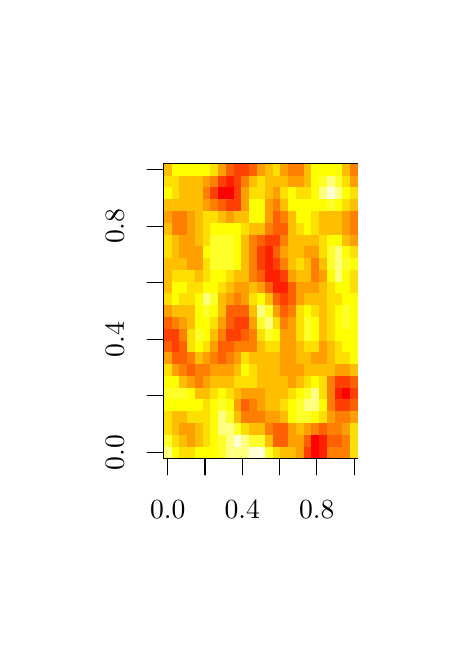
\begin{tikzpicture}[x=1pt,y=1pt]
\definecolor{fillColor}{RGB}{255,255,255}
\path[use as bounding box,fill=fillColor,fill opacity=0.00] (0,0) rectangle (144.54,216.81);
\begin{scope}
\path[clip] (  0.00,  0.00) rectangle (144.54,216.81);
\definecolor{drawColor}{RGB}{0,0,0}

\path[draw=drawColor,line width= 0.4pt,line join=round,line cap=round] ( 50.60, 61.20) -- (117.94, 61.20);

\path[draw=drawColor,line width= 0.4pt,line join=round,line cap=round] ( 50.60, 61.20) -- ( 50.60, 55.20);

\path[draw=drawColor,line width= 0.4pt,line join=round,line cap=round] ( 64.07, 61.20) -- ( 64.07, 55.20);

\path[draw=drawColor,line width= 0.4pt,line join=round,line cap=round] ( 77.54, 61.20) -- ( 77.54, 55.20);

\path[draw=drawColor,line width= 0.4pt,line join=round,line cap=round] ( 91.00, 61.20) -- ( 91.00, 55.20);

\path[draw=drawColor,line width= 0.4pt,line join=round,line cap=round] (104.47, 61.20) -- (104.47, 55.20);

\path[draw=drawColor,line width= 0.4pt,line join=round,line cap=round] (117.94, 61.20) -- (117.94, 55.20);

\node[text=drawColor,anchor=base,inner sep=0pt, outer sep=0pt, scale=  1.00] at ( 50.60, 39.60) {0.0};

\node[text=drawColor,anchor=base,inner sep=0pt, outer sep=0pt, scale=  1.00] at ( 77.54, 39.60) {0.4};

\node[text=drawColor,anchor=base,inner sep=0pt, outer sep=0pt, scale=  1.00] at (104.47, 39.60) {0.8};

\path[draw=drawColor,line width= 0.4pt,line join=round,line cap=round] ( 49.20, 63.33) -- ( 49.20,165.48);

\path[draw=drawColor,line width= 0.4pt,line join=round,line cap=round] ( 49.20, 63.33) -- ( 43.20, 63.33);

\path[draw=drawColor,line width= 0.4pt,line join=round,line cap=round] ( 49.20, 83.76) -- ( 43.20, 83.76);

\path[draw=drawColor,line width= 0.4pt,line join=round,line cap=round] ( 49.20,104.19) -- ( 43.20,104.19);

\path[draw=drawColor,line width= 0.4pt,line join=round,line cap=round] ( 49.20,124.62) -- ( 43.20,124.62);

\path[draw=drawColor,line width= 0.4pt,line join=round,line cap=round] ( 49.20,145.05) -- ( 43.20,145.05);

\path[draw=drawColor,line width= 0.4pt,line join=round,line cap=round] ( 49.20,165.48) -- ( 43.20,165.48);

\node[text=drawColor,rotate= 90.00,anchor=base,inner sep=0pt, outer sep=0pt, scale=  1.00] at ( 34.80, 63.33) {0.0};

\node[text=drawColor,rotate= 90.00,anchor=base,inner sep=0pt, outer sep=0pt, scale=  1.00] at ( 34.80,104.19) {0.4};

\node[text=drawColor,rotate= 90.00,anchor=base,inner sep=0pt, outer sep=0pt, scale=  1.00] at ( 34.80,145.05) {0.8};

\path[draw=drawColor,line width= 0.4pt,line join=round,line cap=round] ( 49.20, 61.20) --
	(119.34, 61.20) --
	(119.34,167.61) --
	( 49.20,167.61) --
	( 49.20, 61.20);
\end{scope}
\begin{scope}
\path[clip] ( 49.20, 61.20) rectangle (119.34,167.61);
\definecolor{fillColor}{RGB}{255,255,128}

\path[fill=fillColor] ( 49.20, 61.20) rectangle ( 52.01, 65.46);
\definecolor{fillColor}{RGB}{255,255,42}

\path[fill=fillColor] ( 49.20, 65.46) rectangle ( 52.01, 69.71);
\definecolor{fillColor}{RGB}{255,223,0}

\path[fill=fillColor] ( 49.20, 69.71) rectangle ( 52.01, 73.97);

\path[fill=fillColor] ( 49.20, 73.97) rectangle ( 52.01, 78.23);
\definecolor{fillColor}{RGB}{255,255,0}

\path[fill=fillColor] ( 49.20, 78.23) rectangle ( 52.01, 82.48);
\definecolor{fillColor}{RGB}{255,255,42}

\path[fill=fillColor] ( 49.20, 82.48) rectangle ( 52.01, 86.74);
\definecolor{fillColor}{RGB}{255,255,0}

\path[fill=fillColor] ( 49.20, 86.74) rectangle ( 52.01, 90.99);
\definecolor{fillColor}{RGB}{255,223,0}

\path[fill=fillColor] ( 49.20, 90.99) rectangle ( 52.01, 95.25);
\definecolor{fillColor}{RGB}{255,159,0}

\path[fill=fillColor] ( 49.20, 95.25) rectangle ( 52.01, 99.51);
\definecolor{fillColor}{RGB}{255,96,0}

\path[fill=fillColor] ( 49.20, 99.51) rectangle ( 52.01,103.76);
\definecolor{fillColor}{RGB}{255,64,0}

\path[fill=fillColor] ( 49.20,103.76) rectangle ( 52.01,108.02);
\definecolor{fillColor}{RGB}{255,96,0}

\path[fill=fillColor] ( 49.20,108.02) rectangle ( 52.01,112.28);
\definecolor{fillColor}{RGB}{255,159,0}

\path[fill=fillColor] ( 49.20,112.28) rectangle ( 52.01,116.53);
\definecolor{fillColor}{RGB}{255,223,0}

\path[fill=fillColor] ( 49.20,116.53) rectangle ( 52.01,120.79);
\definecolor{fillColor}{RGB}{255,191,0}

\path[fill=fillColor] ( 49.20,120.79) rectangle ( 52.01,125.05);

\path[fill=fillColor] ( 49.20,125.05) rectangle ( 52.01,129.30);

\path[fill=fillColor] ( 49.20,129.30) rectangle ( 52.01,133.56);
\definecolor{fillColor}{RGB}{255,223,0}

\path[fill=fillColor] ( 49.20,133.56) rectangle ( 52.01,137.82);

\path[fill=fillColor] ( 49.20,137.82) rectangle ( 52.01,142.07);
\definecolor{fillColor}{RGB}{255,191,0}

\path[fill=fillColor] ( 49.20,142.07) rectangle ( 52.01,146.33);
\definecolor{fillColor}{RGB}{255,159,0}

\path[fill=fillColor] ( 49.20,146.33) rectangle ( 52.01,150.58);
\definecolor{fillColor}{RGB}{255,191,0}

\path[fill=fillColor] ( 49.20,150.58) rectangle ( 52.01,154.84);
\definecolor{fillColor}{RGB}{255,255,0}

\path[fill=fillColor] ( 49.20,154.84) rectangle ( 52.01,159.10);
\definecolor{fillColor}{RGB}{255,223,0}

\path[fill=fillColor] ( 49.20,159.10) rectangle ( 52.01,163.35);
\definecolor{fillColor}{RGB}{255,191,0}

\path[fill=fillColor] ( 49.20,163.35) rectangle ( 52.01,167.61);
\definecolor{fillColor}{RGB}{255,255,0}

\path[fill=fillColor] ( 52.01, 61.20) rectangle ( 54.81, 65.46);
\definecolor{fillColor}{RGB}{255,223,0}

\path[fill=fillColor] ( 52.01, 65.46) rectangle ( 54.81, 69.71);
\definecolor{fillColor}{RGB}{255,191,0}

\path[fill=fillColor] ( 52.01, 69.71) rectangle ( 54.81, 73.97);

\path[fill=fillColor] ( 52.01, 73.97) rectangle ( 54.81, 78.23);
\definecolor{fillColor}{RGB}{255,255,0}

\path[fill=fillColor] ( 52.01, 78.23) rectangle ( 54.81, 82.48);
\definecolor{fillColor}{RGB}{255,255,42}

\path[fill=fillColor] ( 52.01, 82.48) rectangle ( 54.81, 86.74);
\definecolor{fillColor}{RGB}{255,255,0}

\path[fill=fillColor] ( 52.01, 86.74) rectangle ( 54.81, 90.99);
\definecolor{fillColor}{RGB}{255,159,0}

\path[fill=fillColor] ( 52.01, 90.99) rectangle ( 54.81, 95.25);
\definecolor{fillColor}{RGB}{255,96,0}

\path[fill=fillColor] ( 52.01, 95.25) rectangle ( 54.81, 99.51);
\definecolor{fillColor}{RGB}{255,64,0}

\path[fill=fillColor] ( 52.01, 99.51) rectangle ( 54.81,103.76);

\path[fill=fillColor] ( 52.01,103.76) rectangle ( 54.81,108.02);
\definecolor{fillColor}{RGB}{255,128,0}

\path[fill=fillColor] ( 52.01,108.02) rectangle ( 54.81,112.28);
\definecolor{fillColor}{RGB}{255,191,0}

\path[fill=fillColor] ( 52.01,112.28) rectangle ( 54.81,116.53);
\definecolor{fillColor}{RGB}{255,255,0}

\path[fill=fillColor] ( 52.01,116.53) rectangle ( 54.81,120.79);

\path[fill=fillColor] ( 52.01,120.79) rectangle ( 54.81,125.05);
\definecolor{fillColor}{RGB}{255,223,0}

\path[fill=fillColor] ( 52.01,125.05) rectangle ( 54.81,129.30);
\definecolor{fillColor}{RGB}{255,191,0}

\path[fill=fillColor] ( 52.01,129.30) rectangle ( 54.81,133.56);

\path[fill=fillColor] ( 52.01,133.56) rectangle ( 54.81,137.82);

\path[fill=fillColor] ( 52.01,137.82) rectangle ( 54.81,142.07);
\definecolor{fillColor}{RGB}{255,128,0}

\path[fill=fillColor] ( 52.01,142.07) rectangle ( 54.81,146.33);

\path[fill=fillColor] ( 52.01,146.33) rectangle ( 54.81,150.58);
\definecolor{fillColor}{RGB}{255,191,0}

\path[fill=fillColor] ( 52.01,150.58) rectangle ( 54.81,154.84);
\definecolor{fillColor}{RGB}{255,223,0}

\path[fill=fillColor] ( 52.01,154.84) rectangle ( 54.81,159.10);

\path[fill=fillColor] ( 52.01,159.10) rectangle ( 54.81,163.35);
\definecolor{fillColor}{RGB}{255,255,0}

\path[fill=fillColor] ( 52.01,163.35) rectangle ( 54.81,167.61);
\definecolor{fillColor}{RGB}{255,223,0}

\path[fill=fillColor] ( 54.81, 61.20) rectangle ( 57.62, 65.46);
\definecolor{fillColor}{RGB}{255,191,0}

\path[fill=fillColor] ( 54.81, 65.46) rectangle ( 57.62, 69.71);
\definecolor{fillColor}{RGB}{255,159,0}

\path[fill=fillColor] ( 54.81, 69.71) rectangle ( 57.62, 73.97);
\definecolor{fillColor}{RGB}{255,191,0}

\path[fill=fillColor] ( 54.81, 73.97) rectangle ( 57.62, 78.23);
\definecolor{fillColor}{RGB}{255,255,0}

\path[fill=fillColor] ( 54.81, 78.23) rectangle ( 57.62, 82.48);
\definecolor{fillColor}{RGB}{255,255,42}

\path[fill=fillColor] ( 54.81, 82.48) rectangle ( 57.62, 86.74);
\definecolor{fillColor}{RGB}{255,191,0}

\path[fill=fillColor] ( 54.81, 86.74) rectangle ( 57.62, 90.99);
\definecolor{fillColor}{RGB}{255,128,0}

\path[fill=fillColor] ( 54.81, 90.99) rectangle ( 57.62, 95.25);
\definecolor{fillColor}{RGB}{255,96,0}

\path[fill=fillColor] ( 54.81, 95.25) rectangle ( 57.62, 99.51);

\path[fill=fillColor] ( 54.81, 99.51) rectangle ( 57.62,103.76);
\definecolor{fillColor}{RGB}{255,128,0}

\path[fill=fillColor] ( 54.81,103.76) rectangle ( 57.62,108.02);
\definecolor{fillColor}{RGB}{255,159,0}

\path[fill=fillColor] ( 54.81,108.02) rectangle ( 57.62,112.28);
\definecolor{fillColor}{RGB}{255,191,0}

\path[fill=fillColor] ( 54.81,112.28) rectangle ( 57.62,116.53);
\definecolor{fillColor}{RGB}{255,223,0}

\path[fill=fillColor] ( 54.81,116.53) rectangle ( 57.62,120.79);
\definecolor{fillColor}{RGB}{255,255,0}

\path[fill=fillColor] ( 54.81,120.79) rectangle ( 57.62,125.05);
\definecolor{fillColor}{RGB}{255,223,0}

\path[fill=fillColor] ( 54.81,125.05) rectangle ( 57.62,129.30);
\definecolor{fillColor}{RGB}{255,191,0}

\path[fill=fillColor] ( 54.81,129.30) rectangle ( 57.62,133.56);
\definecolor{fillColor}{RGB}{255,159,0}

\path[fill=fillColor] ( 54.81,133.56) rectangle ( 57.62,137.82);

\path[fill=fillColor] ( 54.81,137.82) rectangle ( 57.62,142.07);
\definecolor{fillColor}{RGB}{255,128,0}

\path[fill=fillColor] ( 54.81,142.07) rectangle ( 57.62,146.33);

\path[fill=fillColor] ( 54.81,146.33) rectangle ( 57.62,150.58);
\definecolor{fillColor}{RGB}{255,191,0}

\path[fill=fillColor] ( 54.81,150.58) rectangle ( 57.62,154.84);

\path[fill=fillColor] ( 54.81,154.84) rectangle ( 57.62,159.10);

\path[fill=fillColor] ( 54.81,159.10) rectangle ( 57.62,163.35);
\definecolor{fillColor}{RGB}{255,255,0}

\path[fill=fillColor] ( 54.81,163.35) rectangle ( 57.62,167.61);
\definecolor{fillColor}{RGB}{255,223,0}

\path[fill=fillColor] ( 57.62, 61.20) rectangle ( 60.42, 65.46);
\definecolor{fillColor}{RGB}{255,159,0}

\path[fill=fillColor] ( 57.62, 65.46) rectangle ( 60.42, 69.71);

\path[fill=fillColor] ( 57.62, 69.71) rectangle ( 60.42, 73.97);
\definecolor{fillColor}{RGB}{255,223,0}

\path[fill=fillColor] ( 57.62, 73.97) rectangle ( 60.42, 78.23);
\definecolor{fillColor}{RGB}{255,255,0}

\path[fill=fillColor] ( 57.62, 78.23) rectangle ( 60.42, 82.48);

\path[fill=fillColor] ( 57.62, 82.48) rectangle ( 60.42, 86.74);
\definecolor{fillColor}{RGB}{255,159,0}

\path[fill=fillColor] ( 57.62, 86.74) rectangle ( 60.42, 90.99);
\definecolor{fillColor}{RGB}{255,96,0}

\path[fill=fillColor] ( 57.62, 90.99) rectangle ( 60.42, 95.25);
\definecolor{fillColor}{RGB}{255,128,0}

\path[fill=fillColor] ( 57.62, 95.25) rectangle ( 60.42, 99.51);
\definecolor{fillColor}{RGB}{255,223,0}

\path[fill=fillColor] ( 57.62, 99.51) rectangle ( 60.42,103.76);

\path[fill=fillColor] ( 57.62,103.76) rectangle ( 60.42,108.02);
\definecolor{fillColor}{RGB}{255,191,0}

\path[fill=fillColor] ( 57.62,108.02) rectangle ( 60.42,112.28);

\path[fill=fillColor] ( 57.62,112.28) rectangle ( 60.42,116.53);
\definecolor{fillColor}{RGB}{255,223,0}

\path[fill=fillColor] ( 57.62,116.53) rectangle ( 60.42,120.79);

\path[fill=fillColor] ( 57.62,120.79) rectangle ( 60.42,125.05);

\path[fill=fillColor] ( 57.62,125.05) rectangle ( 60.42,129.30);
\definecolor{fillColor}{RGB}{255,159,0}

\path[fill=fillColor] ( 57.62,129.30) rectangle ( 60.42,133.56);

\path[fill=fillColor] ( 57.62,133.56) rectangle ( 60.42,137.82);

\path[fill=fillColor] ( 57.62,137.82) rectangle ( 60.42,142.07);

\path[fill=fillColor] ( 57.62,142.07) rectangle ( 60.42,146.33);

\path[fill=fillColor] ( 57.62,146.33) rectangle ( 60.42,150.58);
\definecolor{fillColor}{RGB}{255,191,0}

\path[fill=fillColor] ( 57.62,150.58) rectangle ( 60.42,154.84);

\path[fill=fillColor] ( 57.62,154.84) rectangle ( 60.42,159.10);

\path[fill=fillColor] ( 57.62,159.10) rectangle ( 60.42,163.35);
\definecolor{fillColor}{RGB}{255,255,0}

\path[fill=fillColor] ( 57.62,163.35) rectangle ( 60.42,167.61);

\path[fill=fillColor] ( 60.42, 61.20) rectangle ( 63.23, 65.46);
\definecolor{fillColor}{RGB}{255,191,0}

\path[fill=fillColor] ( 60.42, 65.46) rectangle ( 63.23, 69.71);

\path[fill=fillColor] ( 60.42, 69.71) rectangle ( 63.23, 73.97);
\definecolor{fillColor}{RGB}{255,223,0}

\path[fill=fillColor] ( 60.42, 73.97) rectangle ( 63.23, 78.23);
\definecolor{fillColor}{RGB}{255,255,0}

\path[fill=fillColor] ( 60.42, 78.23) rectangle ( 63.23, 82.48);
\definecolor{fillColor}{RGB}{255,191,0}

\path[fill=fillColor] ( 60.42, 82.48) rectangle ( 63.23, 86.74);
\definecolor{fillColor}{RGB}{255,128,0}

\path[fill=fillColor] ( 60.42, 86.74) rectangle ( 63.23, 90.99);

\path[fill=fillColor] ( 60.42, 90.99) rectangle ( 63.23, 95.25);
\definecolor{fillColor}{RGB}{255,191,0}

\path[fill=fillColor] ( 60.42, 95.25) rectangle ( 63.23, 99.51);
\definecolor{fillColor}{RGB}{255,255,0}

\path[fill=fillColor] ( 60.42, 99.51) rectangle ( 63.23,103.76);
\definecolor{fillColor}{RGB}{255,255,42}

\path[fill=fillColor] ( 60.42,103.76) rectangle ( 63.23,108.02);
\definecolor{fillColor}{RGB}{255,255,0}

\path[fill=fillColor] ( 60.42,108.02) rectangle ( 63.23,112.28);

\path[fill=fillColor] ( 60.42,112.28) rectangle ( 63.23,116.53);

\path[fill=fillColor] ( 60.42,116.53) rectangle ( 63.23,120.79);
\definecolor{fillColor}{RGB}{255,223,0}

\path[fill=fillColor] ( 60.42,120.79) rectangle ( 63.23,125.05);
\definecolor{fillColor}{RGB}{255,191,0}

\path[fill=fillColor] ( 60.42,125.05) rectangle ( 63.23,129.30);
\definecolor{fillColor}{RGB}{255,159,0}

\path[fill=fillColor] ( 60.42,129.30) rectangle ( 63.23,133.56);

\path[fill=fillColor] ( 60.42,133.56) rectangle ( 63.23,137.82);
\definecolor{fillColor}{RGB}{255,191,0}

\path[fill=fillColor] ( 60.42,137.82) rectangle ( 63.23,142.07);

\path[fill=fillColor] ( 60.42,142.07) rectangle ( 63.23,146.33);

\path[fill=fillColor] ( 60.42,146.33) rectangle ( 63.23,150.58);

\path[fill=fillColor] ( 60.42,150.58) rectangle ( 63.23,154.84);

\path[fill=fillColor] ( 60.42,154.84) rectangle ( 63.23,159.10);

\path[fill=fillColor] ( 60.42,159.10) rectangle ( 63.23,163.35);
\definecolor{fillColor}{RGB}{255,255,0}

\path[fill=fillColor] ( 60.42,163.35) rectangle ( 63.23,167.61);

\path[fill=fillColor] ( 63.23, 61.20) rectangle ( 66.03, 65.46);
\definecolor{fillColor}{RGB}{255,223,0}

\path[fill=fillColor] ( 63.23, 65.46) rectangle ( 66.03, 69.71);

\path[fill=fillColor] ( 63.23, 69.71) rectangle ( 66.03, 73.97);

\path[fill=fillColor] ( 63.23, 73.97) rectangle ( 66.03, 78.23);

\path[fill=fillColor] ( 63.23, 78.23) rectangle ( 66.03, 82.48);
\definecolor{fillColor}{RGB}{255,191,0}

\path[fill=fillColor] ( 63.23, 82.48) rectangle ( 66.03, 86.74);
\definecolor{fillColor}{RGB}{255,159,0}

\path[fill=fillColor] ( 63.23, 86.74) rectangle ( 66.03, 90.99);
\definecolor{fillColor}{RGB}{255,128,0}

\path[fill=fillColor] ( 63.23, 90.99) rectangle ( 66.03, 95.25);
\definecolor{fillColor}{RGB}{255,159,0}

\path[fill=fillColor] ( 63.23, 95.25) rectangle ( 66.03, 99.51);
\definecolor{fillColor}{RGB}{255,223,0}

\path[fill=fillColor] ( 63.23, 99.51) rectangle ( 66.03,103.76);
\definecolor{fillColor}{RGB}{255,255,0}

\path[fill=fillColor] ( 63.23,103.76) rectangle ( 66.03,108.02);

\path[fill=fillColor] ( 63.23,108.02) rectangle ( 66.03,112.28);
\definecolor{fillColor}{RGB}{255,255,42}

\path[fill=fillColor] ( 63.23,112.28) rectangle ( 66.03,116.53);
\definecolor{fillColor}{RGB}{255,255,128}

\path[fill=fillColor] ( 63.23,116.53) rectangle ( 66.03,120.79);
\definecolor{fillColor}{RGB}{255,255,0}

\path[fill=fillColor] ( 63.23,120.79) rectangle ( 66.03,125.05);
\definecolor{fillColor}{RGB}{255,223,0}

\path[fill=fillColor] ( 63.23,125.05) rectangle ( 66.03,129.30);

\path[fill=fillColor] ( 63.23,129.30) rectangle ( 66.03,133.56);
\definecolor{fillColor}{RGB}{255,255,0}

\path[fill=fillColor] ( 63.23,133.56) rectangle ( 66.03,137.82);
\definecolor{fillColor}{RGB}{255,223,0}

\path[fill=fillColor] ( 63.23,137.82) rectangle ( 66.03,142.07);

\path[fill=fillColor] ( 63.23,142.07) rectangle ( 66.03,146.33);

\path[fill=fillColor] ( 63.23,146.33) rectangle ( 66.03,150.58);
\definecolor{fillColor}{RGB}{255,159,0}

\path[fill=fillColor] ( 63.23,150.58) rectangle ( 66.03,154.84);
\definecolor{fillColor}{RGB}{255,128,0}

\path[fill=fillColor] ( 63.23,154.84) rectangle ( 66.03,159.10);
\definecolor{fillColor}{RGB}{255,159,0}

\path[fill=fillColor] ( 63.23,159.10) rectangle ( 66.03,163.35);
\definecolor{fillColor}{RGB}{255,255,0}

\path[fill=fillColor] ( 63.23,163.35) rectangle ( 66.03,167.61);

\path[fill=fillColor] ( 66.03, 61.20) rectangle ( 68.84, 65.46);

\path[fill=fillColor] ( 66.03, 65.46) rectangle ( 68.84, 69.71);

\path[fill=fillColor] ( 66.03, 69.71) rectangle ( 68.84, 73.97);

\path[fill=fillColor] ( 66.03, 73.97) rectangle ( 68.84, 78.23);

\path[fill=fillColor] ( 66.03, 78.23) rectangle ( 68.84, 82.48);
\definecolor{fillColor}{RGB}{255,223,0}

\path[fill=fillColor] ( 66.03, 82.48) rectangle ( 68.84, 86.74);
\definecolor{fillColor}{RGB}{255,191,0}

\path[fill=fillColor] ( 66.03, 86.74) rectangle ( 68.84, 90.99);
\definecolor{fillColor}{RGB}{255,159,0}

\path[fill=fillColor] ( 66.03, 90.99) rectangle ( 68.84, 95.25);
\definecolor{fillColor}{RGB}{255,128,0}

\path[fill=fillColor] ( 66.03, 95.25) rectangle ( 68.84, 99.51);
\definecolor{fillColor}{RGB}{255,159,0}

\path[fill=fillColor] ( 66.03, 99.51) rectangle ( 68.84,103.76);
\definecolor{fillColor}{RGB}{255,191,0}

\path[fill=fillColor] ( 66.03,103.76) rectangle ( 68.84,108.02);
\definecolor{fillColor}{RGB}{255,223,0}

\path[fill=fillColor] ( 66.03,108.02) rectangle ( 68.84,112.28);
\definecolor{fillColor}{RGB}{255,255,0}

\path[fill=fillColor] ( 66.03,112.28) rectangle ( 68.84,116.53);
\definecolor{fillColor}{RGB}{255,255,42}

\path[fill=fillColor] ( 66.03,116.53) rectangle ( 68.84,120.79);
\definecolor{fillColor}{RGB}{255,255,0}

\path[fill=fillColor] ( 66.03,120.79) rectangle ( 68.84,125.05);

\path[fill=fillColor] ( 66.03,125.05) rectangle ( 68.84,129.30);
\definecolor{fillColor}{RGB}{255,255,42}

\path[fill=fillColor] ( 66.03,129.30) rectangle ( 68.84,133.56);

\path[fill=fillColor] ( 66.03,133.56) rectangle ( 68.84,137.82);

\path[fill=fillColor] ( 66.03,137.82) rectangle ( 68.84,142.07);
\definecolor{fillColor}{RGB}{255,255,0}

\path[fill=fillColor] ( 66.03,142.07) rectangle ( 68.84,146.33);
\definecolor{fillColor}{RGB}{255,223,0}

\path[fill=fillColor] ( 66.03,146.33) rectangle ( 68.84,150.58);
\definecolor{fillColor}{RGB}{255,128,0}

\path[fill=fillColor] ( 66.03,150.58) rectangle ( 68.84,154.84);
\definecolor{fillColor}{RGB}{255,64,0}

\path[fill=fillColor] ( 66.03,154.84) rectangle ( 68.84,159.10);
\definecolor{fillColor}{RGB}{255,128,0}

\path[fill=fillColor] ( 66.03,159.10) rectangle ( 68.84,163.35);
\definecolor{fillColor}{RGB}{255,223,0}

\path[fill=fillColor] ( 66.03,163.35) rectangle ( 68.84,167.61);
\definecolor{fillColor}{RGB}{255,255,42}

\path[fill=fillColor] ( 68.84, 61.20) rectangle ( 71.64, 65.46);

\path[fill=fillColor] ( 68.84, 65.46) rectangle ( 71.64, 69.71);
\definecolor{fillColor}{RGB}{255,255,128}

\path[fill=fillColor] ( 68.84, 69.71) rectangle ( 71.64, 73.97);

\path[fill=fillColor] ( 68.84, 73.97) rectangle ( 71.64, 78.23);
\definecolor{fillColor}{RGB}{255,255,42}

\path[fill=fillColor] ( 68.84, 78.23) rectangle ( 71.64, 82.48);
\definecolor{fillColor}{RGB}{255,255,0}

\path[fill=fillColor] ( 68.84, 82.48) rectangle ( 71.64, 86.74);
\definecolor{fillColor}{RGB}{255,191,0}

\path[fill=fillColor] ( 68.84, 86.74) rectangle ( 71.64, 90.99);
\definecolor{fillColor}{RGB}{255,159,0}

\path[fill=fillColor] ( 68.84, 90.99) rectangle ( 71.64, 95.25);
\definecolor{fillColor}{RGB}{255,96,0}

\path[fill=fillColor] ( 68.84, 95.25) rectangle ( 71.64, 99.51);

\path[fill=fillColor] ( 68.84, 99.51) rectangle ( 71.64,103.76);
\definecolor{fillColor}{RGB}{255,128,0}

\path[fill=fillColor] ( 68.84,103.76) rectangle ( 71.64,108.02);
\definecolor{fillColor}{RGB}{255,159,0}

\path[fill=fillColor] ( 68.84,108.02) rectangle ( 71.64,112.28);
\definecolor{fillColor}{RGB}{255,191,0}

\path[fill=fillColor] ( 68.84,112.28) rectangle ( 71.64,116.53);

\path[fill=fillColor] ( 68.84,116.53) rectangle ( 71.64,120.79);
\definecolor{fillColor}{RGB}{255,223,0}

\path[fill=fillColor] ( 68.84,120.79) rectangle ( 71.64,125.05);
\definecolor{fillColor}{RGB}{255,255,0}

\path[fill=fillColor] ( 68.84,125.05) rectangle ( 71.64,129.30);
\definecolor{fillColor}{RGB}{255,255,42}

\path[fill=fillColor] ( 68.84,129.30) rectangle ( 71.64,133.56);

\path[fill=fillColor] ( 68.84,133.56) rectangle ( 71.64,137.82);

\path[fill=fillColor] ( 68.84,137.82) rectangle ( 71.64,142.07);
\definecolor{fillColor}{RGB}{255,255,0}

\path[fill=fillColor] ( 68.84,142.07) rectangle ( 71.64,146.33);
\definecolor{fillColor}{RGB}{255,191,0}

\path[fill=fillColor] ( 68.84,146.33) rectangle ( 71.64,150.58);
\definecolor{fillColor}{RGB}{255,96,0}

\path[fill=fillColor] ( 68.84,150.58) rectangle ( 71.64,154.84);
\definecolor{fillColor}{RGB}{255,0,0}

\path[fill=fillColor] ( 68.84,154.84) rectangle ( 71.64,159.10);
\definecolor{fillColor}{RGB}{255,64,0}

\path[fill=fillColor] ( 68.84,159.10) rectangle ( 71.64,163.35);
\definecolor{fillColor}{RGB}{255,159,0}

\path[fill=fillColor] ( 68.84,163.35) rectangle ( 71.64,167.61);
\definecolor{fillColor}{RGB}{255,255,128}

\path[fill=fillColor] ( 71.64, 61.20) rectangle ( 74.45, 65.46);

\path[fill=fillColor] ( 71.64, 65.46) rectangle ( 74.45, 69.71);

\path[fill=fillColor] ( 71.64, 69.71) rectangle ( 74.45, 73.97);
\definecolor{fillColor}{RGB}{255,255,42}

\path[fill=fillColor] ( 71.64, 73.97) rectangle ( 74.45, 78.23);
\definecolor{fillColor}{RGB}{255,255,0}

\path[fill=fillColor] ( 71.64, 78.23) rectangle ( 74.45, 82.48);
\definecolor{fillColor}{RGB}{255,223,0}

\path[fill=fillColor] ( 71.64, 82.48) rectangle ( 74.45, 86.74);
\definecolor{fillColor}{RGB}{255,191,0}

\path[fill=fillColor] ( 71.64, 86.74) rectangle ( 74.45, 90.99);
\definecolor{fillColor}{RGB}{255,159,0}

\path[fill=fillColor] ( 71.64, 90.99) rectangle ( 74.45, 95.25);
\definecolor{fillColor}{RGB}{255,128,0}

\path[fill=fillColor] ( 71.64, 95.25) rectangle ( 74.45, 99.51);
\definecolor{fillColor}{RGB}{255,96,0}

\path[fill=fillColor] ( 71.64, 99.51) rectangle ( 74.45,103.76);
\definecolor{fillColor}{RGB}{255,64,0}

\path[fill=fillColor] ( 71.64,103.76) rectangle ( 74.45,108.02);
\definecolor{fillColor}{RGB}{255,96,0}

\path[fill=fillColor] ( 71.64,108.02) rectangle ( 74.45,112.28);

\path[fill=fillColor] ( 71.64,112.28) rectangle ( 74.45,116.53);
\definecolor{fillColor}{RGB}{255,159,0}

\path[fill=fillColor] ( 71.64,116.53) rectangle ( 74.45,120.79);
\definecolor{fillColor}{RGB}{255,191,0}

\path[fill=fillColor] ( 71.64,120.79) rectangle ( 74.45,125.05);
\definecolor{fillColor}{RGB}{255,223,0}

\path[fill=fillColor] ( 71.64,125.05) rectangle ( 74.45,129.30);
\definecolor{fillColor}{RGB}{255,255,42}

\path[fill=fillColor] ( 71.64,129.30) rectangle ( 74.45,133.56);

\path[fill=fillColor] ( 71.64,133.56) rectangle ( 74.45,137.82);

\path[fill=fillColor] ( 71.64,137.82) rectangle ( 74.45,142.07);
\definecolor{fillColor}{RGB}{255,255,0}

\path[fill=fillColor] ( 71.64,142.07) rectangle ( 74.45,146.33);
\definecolor{fillColor}{RGB}{255,159,0}

\path[fill=fillColor] ( 71.64,146.33) rectangle ( 74.45,150.58);
\definecolor{fillColor}{RGB}{255,64,0}

\path[fill=fillColor] ( 71.64,150.58) rectangle ( 74.45,154.84);
\definecolor{fillColor}{RGB}{255,0,0}

\path[fill=fillColor] ( 71.64,154.84) rectangle ( 74.45,159.10);
\definecolor{fillColor}{RGB}{255,32,0}

\path[fill=fillColor] ( 71.64,159.10) rectangle ( 74.45,163.35);
\definecolor{fillColor}{RGB}{255,96,0}

\path[fill=fillColor] ( 71.64,163.35) rectangle ( 74.45,167.61);
\definecolor{fillColor}{RGB}{255,255,128}

\path[fill=fillColor] ( 74.45, 61.20) rectangle ( 77.26, 65.46);
\definecolor{fillColor}{RGB}{255,255,213}

\path[fill=fillColor] ( 74.45, 65.46) rectangle ( 77.26, 69.71);
\definecolor{fillColor}{RGB}{255,255,42}

\path[fill=fillColor] ( 74.45, 69.71) rectangle ( 77.26, 73.97);
\definecolor{fillColor}{RGB}{255,191,0}

\path[fill=fillColor] ( 74.45, 73.97) rectangle ( 77.26, 78.23);
\definecolor{fillColor}{RGB}{255,159,0}

\path[fill=fillColor] ( 74.45, 78.23) rectangle ( 77.26, 82.48);
\definecolor{fillColor}{RGB}{255,191,0}

\path[fill=fillColor] ( 74.45, 82.48) rectangle ( 77.26, 86.74);
\definecolor{fillColor}{RGB}{255,223,0}

\path[fill=fillColor] ( 74.45, 86.74) rectangle ( 77.26, 90.99);
\definecolor{fillColor}{RGB}{255,191,0}

\path[fill=fillColor] ( 74.45, 90.99) rectangle ( 77.26, 95.25);
\definecolor{fillColor}{RGB}{255,159,0}

\path[fill=fillColor] ( 74.45, 95.25) rectangle ( 77.26, 99.51);
\definecolor{fillColor}{RGB}{255,128,0}

\path[fill=fillColor] ( 74.45, 99.51) rectangle ( 77.26,103.76);
\definecolor{fillColor}{RGB}{255,64,0}

\path[fill=fillColor] ( 74.45,103.76) rectangle ( 77.26,108.02);

\path[fill=fillColor] ( 74.45,108.02) rectangle ( 77.26,112.28);
\definecolor{fillColor}{RGB}{255,96,0}

\path[fill=fillColor] ( 74.45,112.28) rectangle ( 77.26,116.53);
\definecolor{fillColor}{RGB}{255,128,0}

\path[fill=fillColor] ( 74.45,116.53) rectangle ( 77.26,120.79);
\definecolor{fillColor}{RGB}{255,159,0}

\path[fill=fillColor] ( 74.45,120.79) rectangle ( 77.26,125.05);
\definecolor{fillColor}{RGB}{255,191,0}

\path[fill=fillColor] ( 74.45,125.05) rectangle ( 77.26,129.30);
\definecolor{fillColor}{RGB}{255,255,0}

\path[fill=fillColor] ( 74.45,129.30) rectangle ( 77.26,133.56);

\path[fill=fillColor] ( 74.45,133.56) rectangle ( 77.26,137.82);

\path[fill=fillColor] ( 74.45,137.82) rectangle ( 77.26,142.07);

\path[fill=fillColor] ( 74.45,142.07) rectangle ( 77.26,146.33);
\definecolor{fillColor}{RGB}{255,191,0}

\path[fill=fillColor] ( 74.45,146.33) rectangle ( 77.26,150.58);
\definecolor{fillColor}{RGB}{255,64,0}

\path[fill=fillColor] ( 74.45,150.58) rectangle ( 77.26,154.84);

\path[fill=fillColor] ( 74.45,154.84) rectangle ( 77.26,159.10);

\path[fill=fillColor] ( 74.45,159.10) rectangle ( 77.26,163.35);

\path[fill=fillColor] ( 74.45,163.35) rectangle ( 77.26,167.61);
\definecolor{fillColor}{RGB}{255,255,128}

\path[fill=fillColor] ( 77.26, 61.20) rectangle ( 80.06, 65.46);

\path[fill=fillColor] ( 77.26, 65.46) rectangle ( 80.06, 69.71);
\definecolor{fillColor}{RGB}{255,223,0}

\path[fill=fillColor] ( 77.26, 69.71) rectangle ( 80.06, 73.97);
\definecolor{fillColor}{RGB}{255,128,0}

\path[fill=fillColor] ( 77.26, 73.97) rectangle ( 80.06, 78.23);
\definecolor{fillColor}{RGB}{255,96,0}

\path[fill=fillColor] ( 77.26, 78.23) rectangle ( 80.06, 82.48);
\definecolor{fillColor}{RGB}{255,159,0}

\path[fill=fillColor] ( 77.26, 82.48) rectangle ( 80.06, 86.74);
\definecolor{fillColor}{RGB}{255,223,0}

\path[fill=fillColor] ( 77.26, 86.74) rectangle ( 80.06, 90.99);
\definecolor{fillColor}{RGB}{255,255,0}

\path[fill=fillColor] ( 77.26, 90.99) rectangle ( 80.06, 95.25);
\definecolor{fillColor}{RGB}{255,223,0}

\path[fill=fillColor] ( 77.26, 95.25) rectangle ( 80.06, 99.51);
\definecolor{fillColor}{RGB}{255,128,0}

\path[fill=fillColor] ( 77.26, 99.51) rectangle ( 80.06,103.76);
\definecolor{fillColor}{RGB}{255,96,0}

\path[fill=fillColor] ( 77.26,103.76) rectangle ( 80.06,108.02);
\definecolor{fillColor}{RGB}{255,64,0}

\path[fill=fillColor] ( 77.26,108.02) rectangle ( 80.06,112.28);
\definecolor{fillColor}{RGB}{255,96,0}

\path[fill=fillColor] ( 77.26,112.28) rectangle ( 80.06,116.53);
\definecolor{fillColor}{RGB}{255,159,0}

\path[fill=fillColor] ( 77.26,116.53) rectangle ( 80.06,120.79);

\path[fill=fillColor] ( 77.26,120.79) rectangle ( 80.06,125.05);
\definecolor{fillColor}{RGB}{255,191,0}

\path[fill=fillColor] ( 77.26,125.05) rectangle ( 80.06,129.30);

\path[fill=fillColor] ( 77.26,129.30) rectangle ( 80.06,133.56);

\path[fill=fillColor] ( 77.26,133.56) rectangle ( 80.06,137.82);

\path[fill=fillColor] ( 77.26,137.82) rectangle ( 80.06,142.07);
\definecolor{fillColor}{RGB}{255,223,0}

\path[fill=fillColor] ( 77.26,142.07) rectangle ( 80.06,146.33);
\definecolor{fillColor}{RGB}{255,191,0}

\path[fill=fillColor] ( 77.26,146.33) rectangle ( 80.06,150.58);
\definecolor{fillColor}{RGB}{255,159,0}

\path[fill=fillColor] ( 77.26,150.58) rectangle ( 80.06,154.84);

\path[fill=fillColor] ( 77.26,154.84) rectangle ( 80.06,159.10);
\definecolor{fillColor}{RGB}{255,128,0}

\path[fill=fillColor] ( 77.26,159.10) rectangle ( 80.06,163.35);
\definecolor{fillColor}{RGB}{255,64,0}

\path[fill=fillColor] ( 77.26,163.35) rectangle ( 80.06,167.61);
\definecolor{fillColor}{RGB}{255,255,213}

\path[fill=fillColor] ( 80.06, 61.20) rectangle ( 82.87, 65.46);
\definecolor{fillColor}{RGB}{255,255,42}

\path[fill=fillColor] ( 80.06, 65.46) rectangle ( 82.87, 69.71);
\definecolor{fillColor}{RGB}{255,191,0}

\path[fill=fillColor] ( 80.06, 69.71) rectangle ( 82.87, 73.97);
\definecolor{fillColor}{RGB}{255,128,0}

\path[fill=fillColor] ( 80.06, 73.97) rectangle ( 82.87, 78.23);

\path[fill=fillColor] ( 80.06, 78.23) rectangle ( 82.87, 82.48);
\definecolor{fillColor}{RGB}{255,159,0}

\path[fill=fillColor] ( 80.06, 82.48) rectangle ( 82.87, 86.74);
\definecolor{fillColor}{RGB}{255,223,0}

\path[fill=fillColor] ( 80.06, 86.74) rectangle ( 82.87, 90.99);

\path[fill=fillColor] ( 80.06, 90.99) rectangle ( 82.87, 95.25);
\definecolor{fillColor}{RGB}{255,191,0}

\path[fill=fillColor] ( 80.06, 95.25) rectangle ( 82.87, 99.51);
\definecolor{fillColor}{RGB}{255,128,0}

\path[fill=fillColor] ( 80.06, 99.51) rectangle ( 82.87,103.76);

\path[fill=fillColor] ( 80.06,103.76) rectangle ( 82.87,108.02);
\definecolor{fillColor}{RGB}{255,159,0}

\path[fill=fillColor] ( 80.06,108.02) rectangle ( 82.87,112.28);
\definecolor{fillColor}{RGB}{255,191,0}

\path[fill=fillColor] ( 80.06,112.28) rectangle ( 82.87,116.53);
\definecolor{fillColor}{RGB}{255,223,0}

\path[fill=fillColor] ( 80.06,116.53) rectangle ( 82.87,120.79);
\definecolor{fillColor}{RGB}{255,191,0}

\path[fill=fillColor] ( 80.06,120.79) rectangle ( 82.87,125.05);
\definecolor{fillColor}{RGB}{255,128,0}

\path[fill=fillColor] ( 80.06,125.05) rectangle ( 82.87,129.30);

\path[fill=fillColor] ( 80.06,129.30) rectangle ( 82.87,133.56);

\path[fill=fillColor] ( 80.06,133.56) rectangle ( 82.87,137.82);

\path[fill=fillColor] ( 80.06,137.82) rectangle ( 82.87,142.07);
\definecolor{fillColor}{RGB}{255,191,0}

\path[fill=fillColor] ( 80.06,142.07) rectangle ( 82.87,146.33);
\definecolor{fillColor}{RGB}{255,255,0}

\path[fill=fillColor] ( 80.06,146.33) rectangle ( 82.87,150.58);

\path[fill=fillColor] ( 80.06,150.58) rectangle ( 82.87,154.84);
\definecolor{fillColor}{RGB}{255,223,0}

\path[fill=fillColor] ( 80.06,154.84) rectangle ( 82.87,159.10);
\definecolor{fillColor}{RGB}{255,191,0}

\path[fill=fillColor] ( 80.06,159.10) rectangle ( 82.87,163.35);
\definecolor{fillColor}{RGB}{255,96,0}

\path[fill=fillColor] ( 80.06,163.35) rectangle ( 82.87,167.61);
\definecolor{fillColor}{RGB}{255,255,213}

\path[fill=fillColor] ( 82.87, 61.20) rectangle ( 85.67, 65.46);
\definecolor{fillColor}{RGB}{255,255,42}

\path[fill=fillColor] ( 82.87, 65.46) rectangle ( 85.67, 69.71);
\definecolor{fillColor}{RGB}{255,191,0}

\path[fill=fillColor] ( 82.87, 69.71) rectangle ( 85.67, 73.97);
\definecolor{fillColor}{RGB}{255,128,0}

\path[fill=fillColor] ( 82.87, 73.97) rectangle ( 85.67, 78.23);
\definecolor{fillColor}{RGB}{255,159,0}

\path[fill=fillColor] ( 82.87, 78.23) rectangle ( 85.67, 82.48);

\path[fill=fillColor] ( 82.87, 82.48) rectangle ( 85.67, 86.74);
\definecolor{fillColor}{RGB}{255,191,0}

\path[fill=fillColor] ( 82.87, 86.74) rectangle ( 85.67, 90.99);

\path[fill=fillColor] ( 82.87, 90.99) rectangle ( 85.67, 95.25);

\path[fill=fillColor] ( 82.87, 95.25) rectangle ( 85.67, 99.51);

\path[fill=fillColor] ( 82.87, 99.51) rectangle ( 85.67,103.76);
\definecolor{fillColor}{RGB}{255,223,0}

\path[fill=fillColor] ( 82.87,103.76) rectangle ( 85.67,108.02);
\definecolor{fillColor}{RGB}{255,255,42}

\path[fill=fillColor] ( 82.87,108.02) rectangle ( 85.67,112.28);
\definecolor{fillColor}{RGB}{255,255,128}

\path[fill=fillColor] ( 82.87,112.28) rectangle ( 85.67,116.53);
\definecolor{fillColor}{RGB}{255,255,0}

\path[fill=fillColor] ( 82.87,116.53) rectangle ( 85.67,120.79);
\definecolor{fillColor}{RGB}{255,159,0}

\path[fill=fillColor] ( 82.87,120.79) rectangle ( 85.67,125.05);
\definecolor{fillColor}{RGB}{255,96,0}

\path[fill=fillColor] ( 82.87,125.05) rectangle ( 85.67,129.30);
\definecolor{fillColor}{RGB}{255,64,0}

\path[fill=fillColor] ( 82.87,129.30) rectangle ( 85.67,133.56);

\path[fill=fillColor] ( 82.87,133.56) rectangle ( 85.67,137.82);
\definecolor{fillColor}{RGB}{255,96,0}

\path[fill=fillColor] ( 82.87,137.82) rectangle ( 85.67,142.07);
\definecolor{fillColor}{RGB}{255,191,0}

\path[fill=fillColor] ( 82.87,142.07) rectangle ( 85.67,146.33);
\definecolor{fillColor}{RGB}{255,255,0}

\path[fill=fillColor] ( 82.87,146.33) rectangle ( 85.67,150.58);

\path[fill=fillColor] ( 82.87,150.58) rectangle ( 85.67,154.84);
\definecolor{fillColor}{RGB}{255,223,0}

\path[fill=fillColor] ( 82.87,154.84) rectangle ( 85.67,159.10);

\path[fill=fillColor] ( 82.87,159.10) rectangle ( 85.67,163.35);
\definecolor{fillColor}{RGB}{255,159,0}

\path[fill=fillColor] ( 82.87,163.35) rectangle ( 85.67,167.61);
\definecolor{fillColor}{RGB}{255,255,42}

\path[fill=fillColor] ( 85.67, 61.20) rectangle ( 88.48, 65.46);
\definecolor{fillColor}{RGB}{255,191,0}

\path[fill=fillColor] ( 85.67, 65.46) rectangle ( 88.48, 69.71);
\definecolor{fillColor}{RGB}{255,128,0}

\path[fill=fillColor] ( 85.67, 69.71) rectangle ( 88.48, 73.97);
\definecolor{fillColor}{RGB}{255,159,0}

\path[fill=fillColor] ( 85.67, 73.97) rectangle ( 88.48, 78.23);
\definecolor{fillColor}{RGB}{255,191,0}

\path[fill=fillColor] ( 85.67, 78.23) rectangle ( 88.48, 82.48);

\path[fill=fillColor] ( 85.67, 82.48) rectangle ( 88.48, 86.74);

\path[fill=fillColor] ( 85.67, 86.74) rectangle ( 88.48, 90.99);

\path[fill=fillColor] ( 85.67, 90.99) rectangle ( 88.48, 95.25);

\path[fill=fillColor] ( 85.67, 95.25) rectangle ( 88.48, 99.51);
\definecolor{fillColor}{RGB}{255,223,0}

\path[fill=fillColor] ( 85.67, 99.51) rectangle ( 88.48,103.76);
\definecolor{fillColor}{RGB}{255,255,42}

\path[fill=fillColor] ( 85.67,103.76) rectangle ( 88.48,108.02);
\definecolor{fillColor}{RGB}{255,255,128}

\path[fill=fillColor] ( 85.67,108.02) rectangle ( 88.48,112.28);
\definecolor{fillColor}{RGB}{255,255,42}

\path[fill=fillColor] ( 85.67,112.28) rectangle ( 88.48,116.53);
\definecolor{fillColor}{RGB}{255,191,0}

\path[fill=fillColor] ( 85.67,116.53) rectangle ( 88.48,120.79);
\definecolor{fillColor}{RGB}{255,96,0}

\path[fill=fillColor] ( 85.67,120.79) rectangle ( 88.48,125.05);
\definecolor{fillColor}{RGB}{255,32,0}

\path[fill=fillColor] ( 85.67,125.05) rectangle ( 88.48,129.30);

\path[fill=fillColor] ( 85.67,129.30) rectangle ( 88.48,133.56);

\path[fill=fillColor] ( 85.67,133.56) rectangle ( 88.48,137.82);
\definecolor{fillColor}{RGB}{255,64,0}

\path[fill=fillColor] ( 85.67,137.82) rectangle ( 88.48,142.07);
\definecolor{fillColor}{RGB}{255,128,0}

\path[fill=fillColor] ( 85.67,142.07) rectangle ( 88.48,146.33);
\definecolor{fillColor}{RGB}{255,159,0}

\path[fill=fillColor] ( 85.67,146.33) rectangle ( 88.48,150.58);

\path[fill=fillColor] ( 85.67,150.58) rectangle ( 88.48,154.84);
\definecolor{fillColor}{RGB}{255,191,0}

\path[fill=fillColor] ( 85.67,154.84) rectangle ( 88.48,159.10);

\path[fill=fillColor] ( 85.67,159.10) rectangle ( 88.48,163.35);

\path[fill=fillColor] ( 85.67,163.35) rectangle ( 88.48,167.61);
\definecolor{fillColor}{RGB}{255,223,0}

\path[fill=fillColor] ( 88.48, 61.20) rectangle ( 91.28, 65.46);
\definecolor{fillColor}{RGB}{255,96,0}

\path[fill=fillColor] ( 88.48, 65.46) rectangle ( 91.28, 69.71);

\path[fill=fillColor] ( 88.48, 69.71) rectangle ( 91.28, 73.97);
\definecolor{fillColor}{RGB}{255,159,0}

\path[fill=fillColor] ( 88.48, 73.97) rectangle ( 91.28, 78.23);
\definecolor{fillColor}{RGB}{255,191,0}

\path[fill=fillColor] ( 88.48, 78.23) rectangle ( 91.28, 82.48);

\path[fill=fillColor] ( 88.48, 82.48) rectangle ( 91.28, 86.74);

\path[fill=fillColor] ( 88.48, 86.74) rectangle ( 91.28, 90.99);

\path[fill=fillColor] ( 88.48, 90.99) rectangle ( 91.28, 95.25);

\path[fill=fillColor] ( 88.48, 95.25) rectangle ( 91.28, 99.51);
\definecolor{fillColor}{RGB}{255,223,0}

\path[fill=fillColor] ( 88.48, 99.51) rectangle ( 91.28,103.76);
\definecolor{fillColor}{RGB}{255,255,0}

\path[fill=fillColor] ( 88.48,103.76) rectangle ( 91.28,108.02);
\definecolor{fillColor}{RGB}{255,223,0}

\path[fill=fillColor] ( 88.48,108.02) rectangle ( 91.28,112.28);
\definecolor{fillColor}{RGB}{255,159,0}

\path[fill=fillColor] ( 88.48,112.28) rectangle ( 91.28,116.53);
\definecolor{fillColor}{RGB}{255,96,0}

\path[fill=fillColor] ( 88.48,116.53) rectangle ( 91.28,120.79);
\definecolor{fillColor}{RGB}{255,32,0}

\path[fill=fillColor] ( 88.48,120.79) rectangle ( 91.28,125.05);

\path[fill=fillColor] ( 88.48,125.05) rectangle ( 91.28,129.30);
\definecolor{fillColor}{RGB}{255,64,0}

\path[fill=fillColor] ( 88.48,129.30) rectangle ( 91.28,133.56);
\definecolor{fillColor}{RGB}{255,96,0}

\path[fill=fillColor] ( 88.48,133.56) rectangle ( 91.28,137.82);
\definecolor{fillColor}{RGB}{255,64,0}

\path[fill=fillColor] ( 88.48,137.82) rectangle ( 91.28,142.07);
\definecolor{fillColor}{RGB}{255,96,0}

\path[fill=fillColor] ( 88.48,142.07) rectangle ( 91.28,146.33);

\path[fill=fillColor] ( 88.48,146.33) rectangle ( 91.28,150.58);
\definecolor{fillColor}{RGB}{255,128,0}

\path[fill=fillColor] ( 88.48,150.58) rectangle ( 91.28,154.84);
\definecolor{fillColor}{RGB}{255,159,0}

\path[fill=fillColor] ( 88.48,154.84) rectangle ( 91.28,159.10);
\definecolor{fillColor}{RGB}{255,191,0}

\path[fill=fillColor] ( 88.48,159.10) rectangle ( 91.28,163.35);
\definecolor{fillColor}{RGB}{255,223,0}

\path[fill=fillColor] ( 88.48,163.35) rectangle ( 91.28,167.61);
\definecolor{fillColor}{RGB}{255,191,0}

\path[fill=fillColor] ( 91.28, 61.20) rectangle ( 94.09, 65.46);
\definecolor{fillColor}{RGB}{255,96,0}

\path[fill=fillColor] ( 91.28, 65.46) rectangle ( 94.09, 69.71);

\path[fill=fillColor] ( 91.28, 69.71) rectangle ( 94.09, 73.97);
\definecolor{fillColor}{RGB}{255,191,0}

\path[fill=fillColor] ( 91.28, 73.97) rectangle ( 94.09, 78.23);
\definecolor{fillColor}{RGB}{255,223,0}

\path[fill=fillColor] ( 91.28, 78.23) rectangle ( 94.09, 82.48);
\definecolor{fillColor}{RGB}{255,191,0}

\path[fill=fillColor] ( 91.28, 82.48) rectangle ( 94.09, 86.74);

\path[fill=fillColor] ( 91.28, 86.74) rectangle ( 94.09, 90.99);
\definecolor{fillColor}{RGB}{255,159,0}

\path[fill=fillColor] ( 91.28, 90.99) rectangle ( 94.09, 95.25);

\path[fill=fillColor] ( 91.28, 95.25) rectangle ( 94.09, 99.51);

\path[fill=fillColor] ( 91.28, 99.51) rectangle ( 94.09,103.76);

\path[fill=fillColor] ( 91.28,103.76) rectangle ( 94.09,108.02);
\definecolor{fillColor}{RGB}{255,128,0}

\path[fill=fillColor] ( 91.28,108.02) rectangle ( 94.09,112.28);
\definecolor{fillColor}{RGB}{255,96,0}

\path[fill=fillColor] ( 91.28,112.28) rectangle ( 94.09,116.53);
\definecolor{fillColor}{RGB}{255,64,0}

\path[fill=fillColor] ( 91.28,116.53) rectangle ( 94.09,120.79);
\definecolor{fillColor}{RGB}{255,32,0}

\path[fill=fillColor] ( 91.28,120.79) rectangle ( 94.09,125.05);
\definecolor{fillColor}{RGB}{255,64,0}

\path[fill=fillColor] ( 91.28,125.05) rectangle ( 94.09,129.30);
\definecolor{fillColor}{RGB}{255,128,0}

\path[fill=fillColor] ( 91.28,129.30) rectangle ( 94.09,133.56);
\definecolor{fillColor}{RGB}{255,159,0}

\path[fill=fillColor] ( 91.28,133.56) rectangle ( 94.09,137.82);
\definecolor{fillColor}{RGB}{255,128,0}

\path[fill=fillColor] ( 91.28,137.82) rectangle ( 94.09,142.07);
\definecolor{fillColor}{RGB}{255,96,0}

\path[fill=fillColor] ( 91.28,142.07) rectangle ( 94.09,146.33);
\definecolor{fillColor}{RGB}{255,128,0}

\path[fill=fillColor] ( 91.28,146.33) rectangle ( 94.09,150.58);
\definecolor{fillColor}{RGB}{255,191,0}

\path[fill=fillColor] ( 91.28,150.58) rectangle ( 94.09,154.84);
\definecolor{fillColor}{RGB}{255,223,0}

\path[fill=fillColor] ( 91.28,154.84) rectangle ( 94.09,159.10);
\definecolor{fillColor}{RGB}{255,191,0}

\path[fill=fillColor] ( 91.28,159.10) rectangle ( 94.09,163.35);
\definecolor{fillColor}{RGB}{255,159,0}

\path[fill=fillColor] ( 91.28,163.35) rectangle ( 94.09,167.61);
\definecolor{fillColor}{RGB}{255,191,0}

\path[fill=fillColor] ( 94.09, 61.20) rectangle ( 96.90, 65.46);
\definecolor{fillColor}{RGB}{255,159,0}

\path[fill=fillColor] ( 94.09, 65.46) rectangle ( 96.90, 69.71);

\path[fill=fillColor] ( 94.09, 69.71) rectangle ( 96.90, 73.97);
\definecolor{fillColor}{RGB}{255,255,0}

\path[fill=fillColor] ( 94.09, 73.97) rectangle ( 96.90, 78.23);

\path[fill=fillColor] ( 94.09, 78.23) rectangle ( 96.90, 82.48);
\definecolor{fillColor}{RGB}{255,223,0}

\path[fill=fillColor] ( 94.09, 82.48) rectangle ( 96.90, 86.74);
\definecolor{fillColor}{RGB}{255,159,0}

\path[fill=fillColor] ( 94.09, 86.74) rectangle ( 96.90, 90.99);

\path[fill=fillColor] ( 94.09, 90.99) rectangle ( 96.90, 95.25);

\path[fill=fillColor] ( 94.09, 95.25) rectangle ( 96.90, 99.51);

\path[fill=fillColor] ( 94.09, 99.51) rectangle ( 96.90,103.76);

\path[fill=fillColor] ( 94.09,103.76) rectangle ( 96.90,108.02);

\path[fill=fillColor] ( 94.09,108.02) rectangle ( 96.90,112.28);
\definecolor{fillColor}{RGB}{255,128,0}

\path[fill=fillColor] ( 94.09,112.28) rectangle ( 96.90,116.53);
\definecolor{fillColor}{RGB}{255,96,0}

\path[fill=fillColor] ( 94.09,116.53) rectangle ( 96.90,120.79);

\path[fill=fillColor] ( 94.09,120.79) rectangle ( 96.90,125.05);
\definecolor{fillColor}{RGB}{255,159,0}

\path[fill=fillColor] ( 94.09,125.05) rectangle ( 96.90,129.30);
\definecolor{fillColor}{RGB}{255,191,0}

\path[fill=fillColor] ( 94.09,129.30) rectangle ( 96.90,133.56);

\path[fill=fillColor] ( 94.09,133.56) rectangle ( 96.90,137.82);

\path[fill=fillColor] ( 94.09,137.82) rectangle ( 96.90,142.07);

\path[fill=fillColor] ( 94.09,142.07) rectangle ( 96.90,146.33);

\path[fill=fillColor] ( 94.09,146.33) rectangle ( 96.90,150.58);
\definecolor{fillColor}{RGB}{255,255,0}

\path[fill=fillColor] ( 94.09,150.58) rectangle ( 96.90,154.84);

\path[fill=fillColor] ( 94.09,154.84) rectangle ( 96.90,159.10);
\definecolor{fillColor}{RGB}{255,159,0}

\path[fill=fillColor] ( 94.09,159.10) rectangle ( 96.90,163.35);
\definecolor{fillColor}{RGB}{255,128,0}

\path[fill=fillColor] ( 94.09,163.35) rectangle ( 96.90,167.61);
\definecolor{fillColor}{RGB}{255,159,0}

\path[fill=fillColor] ( 96.90, 61.20) rectangle ( 99.70, 65.46);

\path[fill=fillColor] ( 96.90, 65.46) rectangle ( 99.70, 69.71);
\definecolor{fillColor}{RGB}{255,191,0}

\path[fill=fillColor] ( 96.90, 69.71) rectangle ( 99.70, 73.97);
\definecolor{fillColor}{RGB}{255,255,42}

\path[fill=fillColor] ( 96.90, 73.97) rectangle ( 99.70, 78.23);

\path[fill=fillColor] ( 96.90, 78.23) rectangle ( 99.70, 82.48);
\definecolor{fillColor}{RGB}{255,255,0}

\path[fill=fillColor] ( 96.90, 82.48) rectangle ( 99.70, 86.74);
\definecolor{fillColor}{RGB}{255,191,0}

\path[fill=fillColor] ( 96.90, 86.74) rectangle ( 99.70, 90.99);
\definecolor{fillColor}{RGB}{255,159,0}

\path[fill=fillColor] ( 96.90, 90.99) rectangle ( 99.70, 95.25);
\definecolor{fillColor}{RGB}{255,191,0}

\path[fill=fillColor] ( 96.90, 95.25) rectangle ( 99.70, 99.51);

\path[fill=fillColor] ( 96.90, 99.51) rectangle ( 99.70,103.76);
\definecolor{fillColor}{RGB}{255,223,0}

\path[fill=fillColor] ( 96.90,103.76) rectangle ( 99.70,108.02);

\path[fill=fillColor] ( 96.90,108.02) rectangle ( 99.70,112.28);

\path[fill=fillColor] ( 96.90,112.28) rectangle ( 99.70,116.53);
\definecolor{fillColor}{RGB}{255,159,0}

\path[fill=fillColor] ( 96.90,116.53) rectangle ( 99.70,120.79);

\path[fill=fillColor] ( 96.90,120.79) rectangle ( 99.70,125.05);
\definecolor{fillColor}{RGB}{255,191,0}

\path[fill=fillColor] ( 96.90,125.05) rectangle ( 99.70,129.30);
\definecolor{fillColor}{RGB}{255,223,0}

\path[fill=fillColor] ( 96.90,129.30) rectangle ( 99.70,133.56);
\definecolor{fillColor}{RGB}{255,191,0}

\path[fill=fillColor] ( 96.90,133.56) rectangle ( 99.70,137.82);

\path[fill=fillColor] ( 96.90,137.82) rectangle ( 99.70,142.07);
\definecolor{fillColor}{RGB}{255,223,0}

\path[fill=fillColor] ( 96.90,142.07) rectangle ( 99.70,146.33);
\definecolor{fillColor}{RGB}{255,255,0}

\path[fill=fillColor] ( 96.90,146.33) rectangle ( 99.70,150.58);

\path[fill=fillColor] ( 96.90,150.58) rectangle ( 99.70,154.84);
\definecolor{fillColor}{RGB}{255,223,0}

\path[fill=fillColor] ( 96.90,154.84) rectangle ( 99.70,159.10);
\definecolor{fillColor}{RGB}{255,159,0}

\path[fill=fillColor] ( 96.90,159.10) rectangle ( 99.70,163.35);
\definecolor{fillColor}{RGB}{255,128,0}

\path[fill=fillColor] ( 96.90,163.35) rectangle ( 99.70,167.61);
\definecolor{fillColor}{RGB}{255,64,0}

\path[fill=fillColor] ( 99.70, 61.20) rectangle (102.51, 65.46);
\definecolor{fillColor}{RGB}{255,96,0}

\path[fill=fillColor] ( 99.70, 65.46) rectangle (102.51, 69.71);
\definecolor{fillColor}{RGB}{255,159,0}

\path[fill=fillColor] ( 99.70, 69.71) rectangle (102.51, 73.97);
\definecolor{fillColor}{RGB}{255,255,42}

\path[fill=fillColor] ( 99.70, 73.97) rectangle (102.51, 78.23);
\definecolor{fillColor}{RGB}{255,255,128}

\path[fill=fillColor] ( 99.70, 78.23) rectangle (102.51, 82.48);
\definecolor{fillColor}{RGB}{255,255,42}

\path[fill=fillColor] ( 99.70, 82.48) rectangle (102.51, 86.74);
\definecolor{fillColor}{RGB}{255,223,0}

\path[fill=fillColor] ( 99.70, 86.74) rectangle (102.51, 90.99);
\definecolor{fillColor}{RGB}{255,191,0}

\path[fill=fillColor] ( 99.70, 90.99) rectangle (102.51, 95.25);

\path[fill=fillColor] ( 99.70, 95.25) rectangle (102.51, 99.51);
\definecolor{fillColor}{RGB}{255,223,0}

\path[fill=fillColor] ( 99.70, 99.51) rectangle (102.51,103.76);
\definecolor{fillColor}{RGB}{255,255,42}

\path[fill=fillColor] ( 99.70,103.76) rectangle (102.51,108.02);

\path[fill=fillColor] ( 99.70,108.02) rectangle (102.51,112.28);
\definecolor{fillColor}{RGB}{255,255,0}

\path[fill=fillColor] ( 99.70,112.28) rectangle (102.51,116.53);
\definecolor{fillColor}{RGB}{255,191,0}

\path[fill=fillColor] ( 99.70,116.53) rectangle (102.51,120.79);
\definecolor{fillColor}{RGB}{255,159,0}

\path[fill=fillColor] ( 99.70,120.79) rectangle (102.51,125.05);
\definecolor{fillColor}{RGB}{255,191,0}

\path[fill=fillColor] ( 99.70,125.05) rectangle (102.51,129.30);

\path[fill=fillColor] ( 99.70,129.30) rectangle (102.51,133.56);
\definecolor{fillColor}{RGB}{255,159,0}

\path[fill=fillColor] ( 99.70,133.56) rectangle (102.51,137.82);
\definecolor{fillColor}{RGB}{255,191,0}

\path[fill=fillColor] ( 99.70,137.82) rectangle (102.51,142.07);
\definecolor{fillColor}{RGB}{255,255,0}

\path[fill=fillColor] ( 99.70,142.07) rectangle (102.51,146.33);

\path[fill=fillColor] ( 99.70,146.33) rectangle (102.51,150.58);

\path[fill=fillColor] ( 99.70,150.58) rectangle (102.51,154.84);
\definecolor{fillColor}{RGB}{255,223,0}

\path[fill=fillColor] ( 99.70,154.84) rectangle (102.51,159.10);
\definecolor{fillColor}{RGB}{255,191,0}

\path[fill=fillColor] ( 99.70,159.10) rectangle (102.51,163.35);

\path[fill=fillColor] ( 99.70,163.35) rectangle (102.51,167.61);
\definecolor{fillColor}{RGB}{255,0,0}

\path[fill=fillColor] (102.51, 61.20) rectangle (105.31, 65.46);

\path[fill=fillColor] (102.51, 65.46) rectangle (105.31, 69.71);
\definecolor{fillColor}{RGB}{255,128,0}

\path[fill=fillColor] (102.51, 69.71) rectangle (105.31, 73.97);
\definecolor{fillColor}{RGB}{255,255,0}

\path[fill=fillColor] (102.51, 73.97) rectangle (105.31, 78.23);
\definecolor{fillColor}{RGB}{255,255,128}

\path[fill=fillColor] (102.51, 78.23) rectangle (105.31, 82.48);

\path[fill=fillColor] (102.51, 82.48) rectangle (105.31, 86.74);
\definecolor{fillColor}{RGB}{255,255,0}

\path[fill=fillColor] (102.51, 86.74) rectangle (105.31, 90.99);
\definecolor{fillColor}{RGB}{255,191,0}

\path[fill=fillColor] (102.51, 90.99) rectangle (105.31, 95.25);
\definecolor{fillColor}{RGB}{255,159,0}

\path[fill=fillColor] (102.51, 95.25) rectangle (105.31, 99.51);
\definecolor{fillColor}{RGB}{255,223,0}

\path[fill=fillColor] (102.51, 99.51) rectangle (105.31,103.76);
\definecolor{fillColor}{RGB}{255,255,0}

\path[fill=fillColor] (102.51,103.76) rectangle (105.31,108.02);

\path[fill=fillColor] (102.51,108.02) rectangle (105.31,112.28);
\definecolor{fillColor}{RGB}{255,223,0}

\path[fill=fillColor] (102.51,112.28) rectangle (105.31,116.53);
\definecolor{fillColor}{RGB}{255,191,0}

\path[fill=fillColor] (102.51,116.53) rectangle (105.31,120.79);
\definecolor{fillColor}{RGB}{255,159,0}

\path[fill=fillColor] (102.51,120.79) rectangle (105.31,125.05);
\definecolor{fillColor}{RGB}{255,128,0}

\path[fill=fillColor] (102.51,125.05) rectangle (105.31,129.30);

\path[fill=fillColor] (102.51,129.30) rectangle (105.31,133.56);
\definecolor{fillColor}{RGB}{255,159,0}

\path[fill=fillColor] (102.51,133.56) rectangle (105.31,137.82);
\definecolor{fillColor}{RGB}{255,191,0}

\path[fill=fillColor] (102.51,137.82) rectangle (105.31,142.07);
\definecolor{fillColor}{RGB}{255,223,0}

\path[fill=fillColor] (102.51,142.07) rectangle (105.31,146.33);

\path[fill=fillColor] (102.51,146.33) rectangle (105.31,150.58);
\definecolor{fillColor}{RGB}{255,255,0}

\path[fill=fillColor] (102.51,150.58) rectangle (105.31,154.84);

\path[fill=fillColor] (102.51,154.84) rectangle (105.31,159.10);

\path[fill=fillColor] (102.51,159.10) rectangle (105.31,163.35);

\path[fill=fillColor] (102.51,163.35) rectangle (105.31,167.61);
\definecolor{fillColor}{RGB}{255,32,0}

\path[fill=fillColor] (105.31, 61.20) rectangle (108.12, 65.46);

\path[fill=fillColor] (105.31, 65.46) rectangle (108.12, 69.71);
\definecolor{fillColor}{RGB}{255,96,0}

\path[fill=fillColor] (105.31, 69.71) rectangle (108.12, 73.97);
\definecolor{fillColor}{RGB}{255,223,0}

\path[fill=fillColor] (105.31, 73.97) rectangle (108.12, 78.23);
\definecolor{fillColor}{RGB}{255,255,0}

\path[fill=fillColor] (105.31, 78.23) rectangle (108.12, 82.48);
\definecolor{fillColor}{RGB}{255,223,0}

\path[fill=fillColor] (105.31, 82.48) rectangle (108.12, 86.74);

\path[fill=fillColor] (105.31, 86.74) rectangle (108.12, 90.99);
\definecolor{fillColor}{RGB}{255,191,0}

\path[fill=fillColor] (105.31, 90.99) rectangle (108.12, 95.25);
\definecolor{fillColor}{RGB}{255,159,0}

\path[fill=fillColor] (105.31, 95.25) rectangle (108.12, 99.51);

\path[fill=fillColor] (105.31, 99.51) rectangle (108.12,103.76);
\definecolor{fillColor}{RGB}{255,191,0}

\path[fill=fillColor] (105.31,103.76) rectangle (108.12,108.02);

\path[fill=fillColor] (105.31,108.02) rectangle (108.12,112.28);

\path[fill=fillColor] (105.31,112.28) rectangle (108.12,116.53);

\path[fill=fillColor] (105.31,116.53) rectangle (108.12,120.79);

\path[fill=fillColor] (105.31,120.79) rectangle (108.12,125.05);
\definecolor{fillColor}{RGB}{255,159,0}

\path[fill=fillColor] (105.31,125.05) rectangle (108.12,129.30);
\definecolor{fillColor}{RGB}{255,191,0}

\path[fill=fillColor] (105.31,129.30) rectangle (108.12,133.56);
\definecolor{fillColor}{RGB}{255,223,0}

\path[fill=fillColor] (105.31,133.56) rectangle (108.12,137.82);

\path[fill=fillColor] (105.31,137.82) rectangle (108.12,142.07);
\definecolor{fillColor}{RGB}{255,191,0}

\path[fill=fillColor] (105.31,142.07) rectangle (108.12,146.33);

\path[fill=fillColor] (105.31,146.33) rectangle (108.12,150.58);
\definecolor{fillColor}{RGB}{255,255,0}

\path[fill=fillColor] (105.31,150.58) rectangle (108.12,154.84);
\definecolor{fillColor}{RGB}{255,255,128}

\path[fill=fillColor] (105.31,154.84) rectangle (108.12,159.10);
\definecolor{fillColor}{RGB}{255,255,42}

\path[fill=fillColor] (105.31,159.10) rectangle (108.12,163.35);
\definecolor{fillColor}{RGB}{255,255,0}

\path[fill=fillColor] (105.31,163.35) rectangle (108.12,167.61);
\definecolor{fillColor}{RGB}{255,128,0}

\path[fill=fillColor] (108.12, 61.20) rectangle (110.92, 65.46);
\definecolor{fillColor}{RGB}{255,96,0}

\path[fill=fillColor] (108.12, 65.46) rectangle (110.92, 69.71);
\definecolor{fillColor}{RGB}{255,128,0}

\path[fill=fillColor] (108.12, 69.71) rectangle (110.92, 73.97);
\definecolor{fillColor}{RGB}{255,159,0}

\path[fill=fillColor] (108.12, 73.97) rectangle (110.92, 78.23);
\definecolor{fillColor}{RGB}{255,128,0}

\path[fill=fillColor] (108.12, 78.23) rectangle (110.92, 82.48);

\path[fill=fillColor] (108.12, 82.48) rectangle (110.92, 86.74);

\path[fill=fillColor] (108.12, 86.74) rectangle (110.92, 90.99);
\definecolor{fillColor}{RGB}{255,191,0}

\path[fill=fillColor] (108.12, 90.99) rectangle (110.92, 95.25);

\path[fill=fillColor] (108.12, 95.25) rectangle (110.92, 99.51);

\path[fill=fillColor] (108.12, 99.51) rectangle (110.92,103.76);
\definecolor{fillColor}{RGB}{255,223,0}

\path[fill=fillColor] (108.12,103.76) rectangle (110.92,108.02);

\path[fill=fillColor] (108.12,108.02) rectangle (110.92,112.28);

\path[fill=fillColor] (108.12,112.28) rectangle (110.92,116.53);

\path[fill=fillColor] (108.12,116.53) rectangle (110.92,120.79);

\path[fill=fillColor] (108.12,120.79) rectangle (110.92,125.05);
\definecolor{fillColor}{RGB}{255,255,0}

\path[fill=fillColor] (108.12,125.05) rectangle (110.92,129.30);
\definecolor{fillColor}{RGB}{255,255,42}

\path[fill=fillColor] (108.12,129.30) rectangle (110.92,133.56);

\path[fill=fillColor] (108.12,133.56) rectangle (110.92,137.82);
\definecolor{fillColor}{RGB}{255,255,0}

\path[fill=fillColor] (108.12,137.82) rectangle (110.92,142.07);
\definecolor{fillColor}{RGB}{255,191,0}

\path[fill=fillColor] (108.12,142.07) rectangle (110.92,146.33);

\path[fill=fillColor] (108.12,146.33) rectangle (110.92,150.58);
\definecolor{fillColor}{RGB}{255,255,42}

\path[fill=fillColor] (108.12,150.58) rectangle (110.92,154.84);
\definecolor{fillColor}{RGB}{255,255,213}

\path[fill=fillColor] (108.12,154.84) rectangle (110.92,159.10);
\definecolor{fillColor}{RGB}{255,255,128}

\path[fill=fillColor] (108.12,159.10) rectangle (110.92,163.35);
\definecolor{fillColor}{RGB}{255,255,0}

\path[fill=fillColor] (108.12,163.35) rectangle (110.92,167.61);
\definecolor{fillColor}{RGB}{255,128,0}

\path[fill=fillColor] (110.92, 61.20) rectangle (113.73, 65.46);
\definecolor{fillColor}{RGB}{255,96,0}

\path[fill=fillColor] (110.92, 65.46) rectangle (113.73, 69.71);
\definecolor{fillColor}{RGB}{255,128,0}

\path[fill=fillColor] (110.92, 69.71) rectangle (113.73, 73.97);

\path[fill=fillColor] (110.92, 73.97) rectangle (113.73, 78.23);
\definecolor{fillColor}{RGB}{255,64,0}

\path[fill=fillColor] (110.92, 78.23) rectangle (113.73, 82.48);
\definecolor{fillColor}{RGB}{255,32,0}

\path[fill=fillColor] (110.92, 82.48) rectangle (113.73, 86.74);
\definecolor{fillColor}{RGB}{255,64,0}

\path[fill=fillColor] (110.92, 86.74) rectangle (113.73, 90.99);
\definecolor{fillColor}{RGB}{255,159,0}

\path[fill=fillColor] (110.92, 90.99) rectangle (113.73, 95.25);
\definecolor{fillColor}{RGB}{255,223,0}

\path[fill=fillColor] (110.92, 95.25) rectangle (113.73, 99.51);

\path[fill=fillColor] (110.92, 99.51) rectangle (113.73,103.76);
\definecolor{fillColor}{RGB}{255,255,0}

\path[fill=fillColor] (110.92,103.76) rectangle (113.73,108.02);

\path[fill=fillColor] (110.92,108.02) rectangle (113.73,112.28);

\path[fill=fillColor] (110.92,112.28) rectangle (113.73,116.53);
\definecolor{fillColor}{RGB}{255,223,0}

\path[fill=fillColor] (110.92,116.53) rectangle (113.73,120.79);
\definecolor{fillColor}{RGB}{255,255,0}

\path[fill=fillColor] (110.92,120.79) rectangle (113.73,125.05);
\definecolor{fillColor}{RGB}{255,255,128}

\path[fill=fillColor] (110.92,125.05) rectangle (113.73,129.30);

\path[fill=fillColor] (110.92,129.30) rectangle (113.73,133.56);

\path[fill=fillColor] (110.92,133.56) rectangle (113.73,137.82);
\definecolor{fillColor}{RGB}{255,255,0}

\path[fill=fillColor] (110.92,137.82) rectangle (113.73,142.07);
\definecolor{fillColor}{RGB}{255,191,0}

\path[fill=fillColor] (110.92,142.07) rectangle (113.73,146.33);

\path[fill=fillColor] (110.92,146.33) rectangle (113.73,150.58);
\definecolor{fillColor}{RGB}{255,255,0}

\path[fill=fillColor] (110.92,150.58) rectangle (113.73,154.84);
\definecolor{fillColor}{RGB}{255,255,128}

\path[fill=fillColor] (110.92,154.84) rectangle (113.73,159.10);
\definecolor{fillColor}{RGB}{255,255,42}

\path[fill=fillColor] (110.92,159.10) rectangle (113.73,163.35);
\definecolor{fillColor}{RGB}{255,255,0}

\path[fill=fillColor] (110.92,163.35) rectangle (113.73,167.61);
\definecolor{fillColor}{RGB}{255,128,0}

\path[fill=fillColor] (113.73, 61.20) rectangle (116.53, 65.46);

\path[fill=fillColor] (113.73, 65.46) rectangle (116.53, 69.71);
\definecolor{fillColor}{RGB}{255,159,0}

\path[fill=fillColor] (113.73, 69.71) rectangle (116.53, 73.97);
\definecolor{fillColor}{RGB}{255,128,0}

\path[fill=fillColor] (113.73, 73.97) rectangle (116.53, 78.23);
\definecolor{fillColor}{RGB}{255,64,0}

\path[fill=fillColor] (113.73, 78.23) rectangle (116.53, 82.48);
\definecolor{fillColor}{RGB}{255,0,0}

\path[fill=fillColor] (113.73, 82.48) rectangle (116.53, 86.74);
\definecolor{fillColor}{RGB}{255,64,0}

\path[fill=fillColor] (113.73, 86.74) rectangle (116.53, 90.99);
\definecolor{fillColor}{RGB}{255,159,0}

\path[fill=fillColor] (113.73, 90.99) rectangle (116.53, 95.25);
\definecolor{fillColor}{RGB}{255,223,0}

\path[fill=fillColor] (113.73, 95.25) rectangle (116.53, 99.51);
\definecolor{fillColor}{RGB}{255,255,0}

\path[fill=fillColor] (113.73, 99.51) rectangle (116.53,103.76);

\path[fill=fillColor] (113.73,103.76) rectangle (116.53,108.02);
\definecolor{fillColor}{RGB}{255,255,42}

\path[fill=fillColor] (113.73,108.02) rectangle (116.53,112.28);

\path[fill=fillColor] (113.73,112.28) rectangle (116.53,116.53);
\definecolor{fillColor}{RGB}{255,255,0}

\path[fill=fillColor] (113.73,116.53) rectangle (116.53,120.79);

\path[fill=fillColor] (113.73,120.79) rectangle (116.53,125.05);

\path[fill=fillColor] (113.73,125.05) rectangle (116.53,129.30);
\definecolor{fillColor}{RGB}{255,255,42}

\path[fill=fillColor] (113.73,129.30) rectangle (116.53,133.56);
\definecolor{fillColor}{RGB}{255,255,0}

\path[fill=fillColor] (113.73,133.56) rectangle (116.53,137.82);
\definecolor{fillColor}{RGB}{255,191,0}

\path[fill=fillColor] (113.73,137.82) rectangle (116.53,142.07);
\definecolor{fillColor}{RGB}{255,159,0}

\path[fill=fillColor] (113.73,142.07) rectangle (116.53,146.33);

\path[fill=fillColor] (113.73,146.33) rectangle (116.53,150.58);
\definecolor{fillColor}{RGB}{255,223,0}

\path[fill=fillColor] (113.73,150.58) rectangle (116.53,154.84);
\definecolor{fillColor}{RGB}{255,255,0}

\path[fill=fillColor] (113.73,154.84) rectangle (116.53,159.10);
\definecolor{fillColor}{RGB}{255,223,0}

\path[fill=fillColor] (113.73,159.10) rectangle (116.53,163.35);
\definecolor{fillColor}{RGB}{255,191,0}

\path[fill=fillColor] (113.73,163.35) rectangle (116.53,167.61);
\definecolor{fillColor}{RGB}{255,223,0}

\path[fill=fillColor] (116.53, 61.20) rectangle (119.34, 65.46);

\path[fill=fillColor] (116.53, 65.46) rectangle (119.34, 69.71);

\path[fill=fillColor] (116.53, 69.71) rectangle (119.34, 73.97);
\definecolor{fillColor}{RGB}{255,159,0}

\path[fill=fillColor] (116.53, 73.97) rectangle (119.34, 78.23);
\definecolor{fillColor}{RGB}{255,96,0}

\path[fill=fillColor] (116.53, 78.23) rectangle (119.34, 82.48);
\definecolor{fillColor}{RGB}{255,64,0}

\path[fill=fillColor] (116.53, 82.48) rectangle (119.34, 86.74);
\definecolor{fillColor}{RGB}{255,96,0}

\path[fill=fillColor] (116.53, 86.74) rectangle (119.34, 90.99);
\definecolor{fillColor}{RGB}{255,191,0}

\path[fill=fillColor] (116.53, 90.99) rectangle (119.34, 95.25);
\definecolor{fillColor}{RGB}{255,255,0}

\path[fill=fillColor] (116.53, 95.25) rectangle (119.34, 99.51);

\path[fill=fillColor] (116.53, 99.51) rectangle (119.34,103.76);

\path[fill=fillColor] (116.53,103.76) rectangle (119.34,108.02);

\path[fill=fillColor] (116.53,108.02) rectangle (119.34,112.28);

\path[fill=fillColor] (116.53,112.28) rectangle (119.34,116.53);

\path[fill=fillColor] (116.53,116.53) rectangle (119.34,120.79);
\definecolor{fillColor}{RGB}{255,223,0}

\path[fill=fillColor] (116.53,120.79) rectangle (119.34,125.05);

\path[fill=fillColor] (116.53,125.05) rectangle (119.34,129.30);
\definecolor{fillColor}{RGB}{255,255,0}

\path[fill=fillColor] (116.53,129.30) rectangle (119.34,133.56);
\definecolor{fillColor}{RGB}{255,223,0}

\path[fill=fillColor] (116.53,133.56) rectangle (119.34,137.82);
\definecolor{fillColor}{RGB}{255,159,0}

\path[fill=fillColor] (116.53,137.82) rectangle (119.34,142.07);
\definecolor{fillColor}{RGB}{255,128,0}

\path[fill=fillColor] (116.53,142.07) rectangle (119.34,146.33);

\path[fill=fillColor] (116.53,146.33) rectangle (119.34,150.58);
\definecolor{fillColor}{RGB}{255,191,0}

\path[fill=fillColor] (116.53,150.58) rectangle (119.34,154.84);
\definecolor{fillColor}{RGB}{255,223,0}

\path[fill=fillColor] (116.53,154.84) rectangle (119.34,159.10);
\definecolor{fillColor}{RGB}{255,159,0}

\path[fill=fillColor] (116.53,159.10) rectangle (119.34,163.35);
\definecolor{fillColor}{RGB}{255,128,0}

\path[fill=fillColor] (116.53,163.35) rectangle (119.34,167.61);
\end{scope}
\end{tikzpicture}

We simulate three independent replications of an isotropic Gaussian process with $\Signal:\Omega\to(\Pop=[0,1]^2\to\mathbb{R})$, with $\forall \position\in\Pop$, $\mathrm{\mu}[\position]=0$, with a Gaussian Covariogram \eqref{def:gaussiancovariogram} with deviation parameter
 $\parampop_1=1$, and scale parameter $\parampop_2=\lbrace 0.01, 0.1, 1\rbrace$, respectively.
Figure \ref{fig:oaijsfdoij} represents independent realizations of $\Signal$.
\begin{figure}[H]
%\begin{mdframed}
    \caption{Heat maps of realisations of the random process $\Signal:\Omega\to(\Pop=[0,1]^2\to\mathbb{R})$ for different values of $\parampop_2$. For each realisation $\signal$ of the random process $\Signal$, for each $\position$ in $\Pop$, the value of $\signal[\position]$ is color coded with a grayscale gradient.}
    \label{fig:oaijsfdoij}
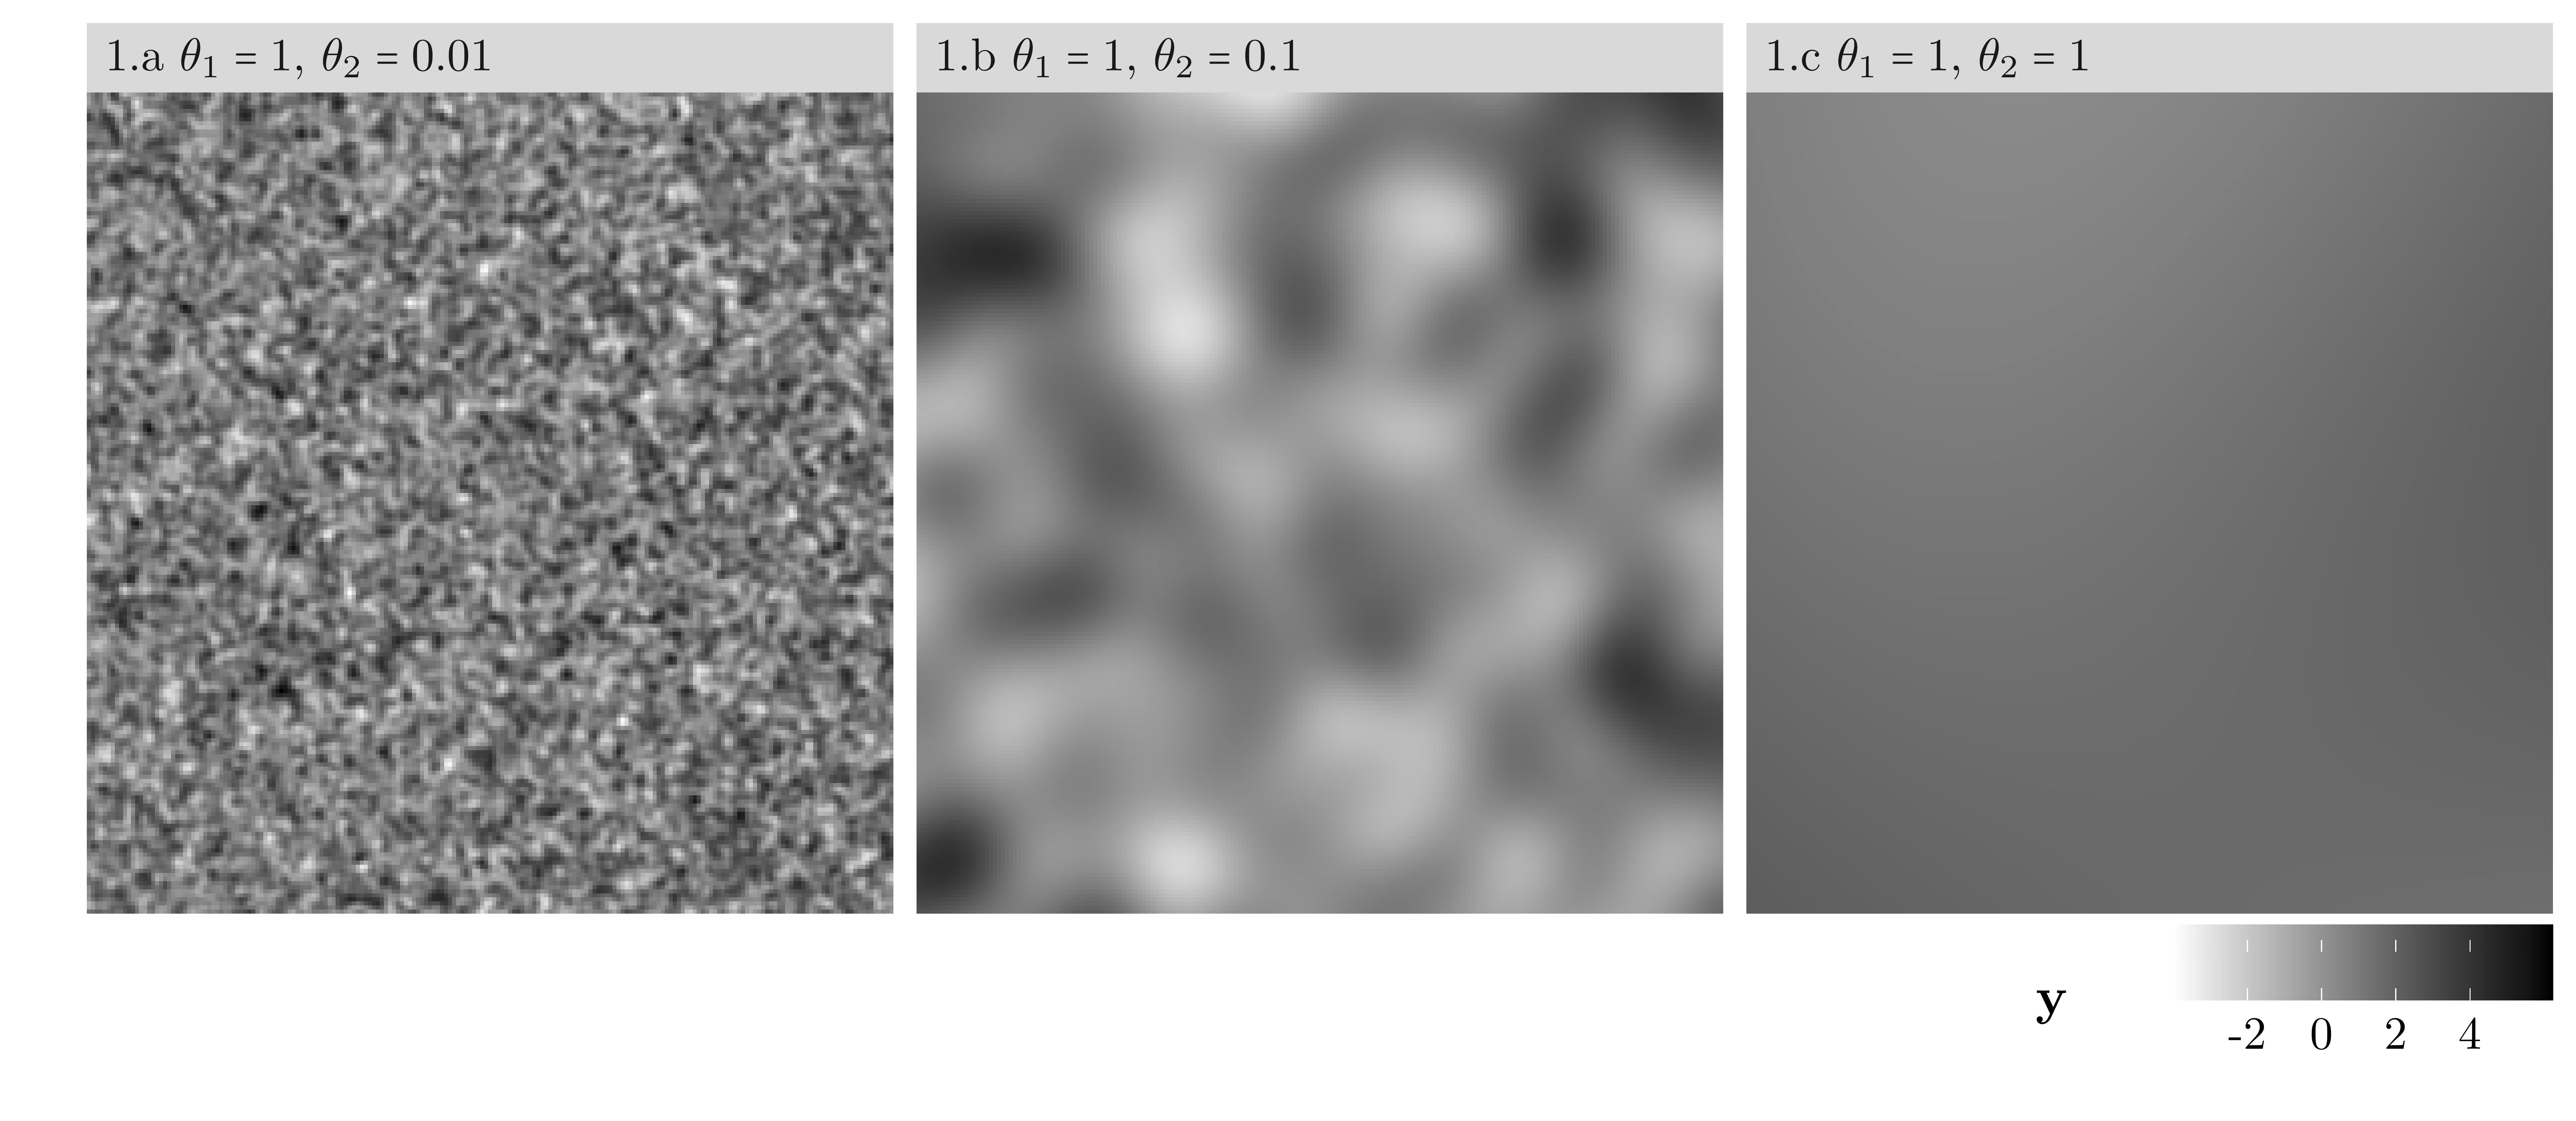
\includegraphics{fig/figure1.png}
%\end{mdframed}
\end{figure}

\end{example}


\subsection{Sample, design and design variable} \label{sec:design}
\subsubsection{Fixed  design variables and fixed designs}
By definition, a fixed design $\design$ is a probability distribution on $\toPop$.
A sample $\Sample$ drawn from $\design$ is a random variable or point process of distribution $\design$, e.g. a random variable $\Sample$ such that $\mathrm{P}^\Sample=\design$. 
Define the size $\Samplesize=\mathrm{size}\circ\Sample$ of the sample $\Sample$. The sample density with respect to $\dominantUbar$ is defined by:
$(\derive P^\Sample)/(\derive\dominantUbar)(\position)=P(N=n)\times(\derive P^{\Sample\mid N=n})/(\derive\dominantU^{\otimes\{1,\ldots,n\}})(\position)$, if $\position\in\Pop^{\{1,\ldots,n\}}$, $P(N=0)$ if $\position=\mathbf{0}$. 
%For example, let $\intensity:(\Pop,\dominantU)\to(\mathbb{R}^+,\mathrm{Lebesgues}(\mathbb{R}^+))$ be a measurable function , then a Poisson point process \citep[p.~ 45]{CoxIshamPointProcesses}) with intensity $\pi$ follows a finite or discrete design if the support of $\dominantU$ is finite. The distribution of a Poisson process when the support of $\dominantU$ is finite is a design that corresponds to with replacement sampling. Confusingly, in the literature on survey sampling, Poisson sampling \citep[p.~85]{SarndalSwensonWretman1992} corresponds to a finite design where each unit $\position$ such that $\pi(\position)>0$ is drawn independently with a fixed probability $\pi(\position)$, and is thus a without replacement design.
A fixed design variable is a function $\desvar:\Pop\mapsto \DesvarSpace$.
A fixed  design $\design$ is usually defined as a function of a fixed design variable and characterized by its density with respect to $\dominantUbar$. For example, the Probability Proportional to Size $\desvar$ With Replacement and size $n$ design, with $\DesvarSpace=[0,+\infty)$, for $\position\in \toPop$, is characterized by:  
\begin{equation}\label{eq:ppswr}\density_{\Sample}(\position)=\left(\derive P^{\Sample}/\derive\dominantUbar\right)(\position)=\left|\begin{array}{l}\left(\int_U \left(\desvar(\position')\right)\mathrm{d}\dominantU (\position')\right)^{-\samplesize}
\left(\prod_{\ell=1}^\samplesize\left(\desvar(\position(\ell))\right)\right)\text{ if }\position\in\Pop^{\{1,\ldots,n\}},\\~0\text{ otherwise.}
\end{array}\right.\end{equation}

We remind that with our notation, $(\desvar.\dominantU)(\Pop)=\int_\Pop \desvar(\position)\derive \dominantU(\position)$. The point process $\Sample$ characterized by Equation \eqref{eq:ppswr} is a binomial point process of $\samplesize$ points in $\Pop$ with intensity $\Pop\to\mathbb{R}, \position\to\left(\left(\desvar.\dominantU\right)\left(\Pop\right)\right)^{-1}\desvar(\position)$, which we abbreviate by $\Sample\sim\mathrm{bpp}\left(\desvar,\samplesize\right)$. Simple random sampling with replacement is a binomial point process with a constant intensity,  and we refer to as $\Sample\sim\mathrm{bpp}\left(1,\samplesize\right)$.  %Pdesigns such that: 
%This general definition includes design for with and without replacement sampling and fixed and random size sampling. 
For example, given a measurable real function $\desvar :\Pop \to\mathbb{R}$, a spatial Poisson Process of intensity $\desvar$ is a point process 
$S:\Omega\to\bigcup_{\samplesize\in\mathbb{N}}\Pop^{\samplesize}$, such that 
for all $\dominantU$-measurable subset $\subsetA$ of $\Pop$, \begin{equation}\label{eq:poissonprocess}
S\sim\mathrm{Ppp}(\desvar)\Leftrightarrow
\mathrm{cardinality}(\Sample^{-1}[\subsetA])\sim \mathrm{Poisson}\left((\desvar.\dominantU)\left(\subsetA \right)\right),
\end{equation}
where $\Sample^{-1}[\subsetA]$ is the random variable with domain the finite subsets of $\Pop$ defined by: $\omega\mapsto\{\ell\in\{1,\ldots,\Samplesize(\omega)\};(\Sample(\omega))(\ell)\in \subsetA\}$ if $\Samplesize(\omega)>0$, $\emptyset$ otherwise. The density of such process with respect to $\bar\dominantU$ is defined, for $\position\in \toPop$, by:
\begin{equation}
\density_{\Sample}(\position)=\left(\derive P^{\Sample}/\derive\dominantUbar\right)(\position)=\left(\size (\position)!\right)^{-1}\exp\left(-\left(\desvar.\dominantU\right)(\Pop)\right)
\prod_{\ell\in\mathrm{domain}(\position)}
\desvar(\position(\ell)).
\end{equation}

For a point process $\Sample$ with values in the measured space $(\Pop,\dominantU)$, for a random variable $W$, define $\Intensity_{S\mid W=w}$ as the intensity measure of $\Sample$ conditionally to $W=w$ with respect to the measure on $\Pop$, where for each measurable subset $\subsetA$ of $\Pop$, $\Intensity_S(A)=\mathrm{E[\mathrm{cardinality}(S^{-1}[A])\mid W=w]}$, and $\intensity_S$ as the density of $\Intensity_S$ with respect to $\dominantU$: $\intensity_S=\derive\Intensity_S/\derive\dominantU$.

%
%The Poisson Point process is such that for two measurable subsets $\subsetA_1$ and $\subsetA_1$  of $\Pop$, 
%$\subsetA_1\cap\subsetA_2=\emptyset\Rightarrow \left(\mathrm{\cardinality}(\subsetA_1\cap\Sample)\perp\mathrm{\cardinality}(\subsetA_2\cap\Sample))$, which is not necessarily the case for each Point Process (for example fixed strictly positive size point processes

%When there exists $\position(1),\ldots,\position_N\in\Pop$ such that $\dominantU=\mathrm{Dirac}_{\{\position(1),\ldots,\position_N}\}$, simple random sampling is  is finite and 

%
%Tables {\ref{tab:oiurhgoieruhgierug}} and 
%\ref{tab:oijgoirejoier} provide examples of continuous and finite population designs. 
%%Notice that the same name is used in the literature for finite or continuous population designs, without contradiction. We put them there as one goal is to establish a parallel between existing theoretical work between finite population and continuous population sampling.
%
%\begin{table}[H]\label{tab:oiurhgoieruhgierug}
%\caption{Continuous population fixed size designs}
%
%\small
%\setlength{\tabcolsep}{8pt}
%\renewcommand{\arraystretch}{1.8}
%
%\newcolumntype{b}{X}
%\newcolumntype{s}{>{\hsize=.1\hsize}X}
%
%\begin{tabularx}{\textwidth}[t]{ssb}
%\hline
%\multicolumn{3}{p{\dimexpr\linewidth-\tabcolsep-\arrayrulewidth}}{Name}\\                 &$\DesvarSpace$ & $\mathrm{d} P^{\Sample[\{1,\ldots,n\}]}/\mathrm{d}\dominantU^{\otimes n}(\position)$\\
%\hline
%\hline
%\multicolumn{3}{p{\dimexpr\linewidth-\tabcolsep-\arrayrulewidth}}{Probability Proportional to Size $\desvar$ With Replacement (PPSWR)}\\                 & $[0,+\infty)$ & $\left(\int_U \left(\desvar(\position']\right)\mathrm{d}\dominantU (\position')\right)^{-n}
%\left(\prod_{\ell=1}^n\left(\desvar(\position(\ell)]\right)\right)$\\
%\hline 
%\multicolumn{3}{p{\dimexpr\linewidth-\tabcolsep-\arrayrulewidth}}{Sytematic sampling, $\samplesize=(n')^2$ }\\&$\{1\}$                 &
%$\left\{\begin{array}{ll}(n!)^{-1} n &\text{ if }\position\in\left\{(\position_0+(n')^{-1}\paramnuisance_0)_{\paramnuisance_0\in \{0,\ldots,n'-1\}^2}\mid\position_0\in [0,1/n']^2\right\}\\0& \text{ otherwise.}\end{array}\right.$\\
%\hline 
%\multicolumn{3}{p{\dimexpr\linewidth-\tabcolsep-\arrayrulewidth}}{Simple Random Sampling}\\                 & ${1}$ & $\dominantU^{}\left(\int_\Delta \left(\desvar(\position']\right)\mathrm{d} (\position')\right)^{-n}
%\mathds{1}_\Delta(\position)$\\
%\hline 
%\end{tabularx}
%
%\end{table}
%
%
%\begin{table}[H] \label{tab:oijgoirejoier}
%\caption{Finite population fixed size  designs}
%
%
%\setlength{\tabcolsep}{8pt}
%\renewcommand{\arraystretch}{1.8}
%
%\begin{tabular}{lll}
%\hline
%Name                 &$\DesvarSpace$ & $\mathrm{d} P^{\Sample[\{1,\ldots,n\}]}/\mathrm{d}\dominantU^{\otimes n}(\position)$\\
%\hline
%\hline
%PPSWR &$\mathbb{R}^+$ & $\left(\int_U \Desvar[\position']\mathrm{d}\dominantU (\position')\right)^{-n}
%\left(\prod_{\ell=1}^n\Desvar[\position(\ell)]\right)$\\
%\end{tabular}
%\end{table}


\subsubsection{Random design variables and random designs}
In practice, the design parameter $\desvar$ is modeled as the output of a random process $\Desvar:\Omega\to(\Pop\to \DesvarSpace)$ that we will refer to as the design variable.
The selection process, when controlled, is in practice a function of an auxiliary variable, called design variable, that is a process defined on the same space $\Pop$. When the selection process is not chosen by the experimenter it can also be modelled as a function of such a process that can be observed, partially observed or latent. In practice, it may not be reasonable to assume independence of the design variable  $\Desvar$ and study variable $\Signal$.


The design $\Design$ is by definition a random variable with domain the set of probability distributions on  $\toPop$. The sample is a random variable $\Sample$ with domain $\toPop$ such that the distribution of $\Sample$ conditionally to the design \emph{is} the design, e.g:
\begin{equation}P^\Design-a.s.(\design),~P^{\Sample\mid \Design=\design}=\design.\end{equation}

We assume that the distribution of the sample conditionally on the design, the signal and the design variable is the design:
\begin{equation}\label{eq:SconditionalonDindependentonYZ}
P^{\Design,\Signal,\Desvar}-a.s.(\design,\signal,\desvar),~P^{\Sample\mid \Design=\design,\Signal=\signal,\Desvar=\desvar}=\design.\end{equation}
This assumption is an independence of the sample $\Sample$ on the design variable and the signal conditionally on the design, which does not imply independence of the sample and the signal.

%In the following, we assume that $P^\Desvar$ is such that $P^\Sample$ is the  uniform distribution on $\Pop^n$: unconditionally on $Z$, the selection is uniform <<< this is wrong.

%We also assume that the design follows the following exchangeability condition: for all $\samplesize\in\mathbb{N}$, for any permutation $\sigma$ of $\{1,\ldots,n\}$, for all measurable subset A of $(\{1,\ldots,n\}\to \Pop)$, for all $\omega\in\Omega$,
%$D(\omega)(A)=D(\omega)(\sigma.A)$, where $\sigma.A(k)=A(\sigma(k))$. 

%\subsubsection{Sample indicator}
%
%The sample indicator is the random variable $I$ defined by: for a subset $A$ of $\Pop$, $I[A]=1$ if $A\subset \Sample$, $0$ otherwise.

 For simplicity, we only consider exchangeable index sample designs, in the sense that $\forall \samplesize\in\mathbb{N}$, for all permutation $\permutation$ of $\{1,\ldots,n\}$,
 \begin{equation}P^\Desvar-\text{a.s.}(\desvar), P^{S\mid\Samplesize=\samplesize,\Desvar=\desvar}=P^{S[\permutation]\mid \Samplesize=\samplesize,\Desvar=\desvar}\label{assumption:designindexexchangeability}.\end{equation}
which ensures that 
 \begin{equation}P^{S\mid\Samplesize=\samplesize}=P^{S[\permutation]\mid \Samplesize=\samplesize}\label{assumption:designindexexchangeability}.\end{equation}


\begin{example}[Example \ref{example:main} continued: distribution of $\Desvar$ conditionally on $\Signal$]
\label{example:2.2}
We assume that 
$\Desvar$ satisfies:
$$\Desvar=\mathrm{exp}\left(\paramnuisance_0+\paramnuisance_1\Signal+\paramnuisance_2 \varepsilon\right),$$
where $\paramnuisance_0$,  $\paramnuisance_1$, $\paramnuisance_2$ are real positive numbers, 
$\varepsilon:\Omega\to\left(\Pop\to\mathbb{R}\right)$
is an isotropic Gaussian process with mean
$\mu=0$ and Gaussian covariogram $\Covariogram(h)=\exp\left(-\|h\|^2/\paramnuisance_{\text{scale}}^2)\right)$ with scale parameter $\paramnuisance_{\text{scale}}=0.1$. The variable $\signal:\Pop\to\mathbb{R}$ (resp $e:\Pop\to\mathbb{R}$) is generated once by sampling from $\Signal$ (resp $\varepsilon$). The variable $\desvar=\exp\left(\paramnuisance_0+\paramnuisance_1\signal+\paramnuisance_2\mathbf{e}\right)$ is computed for 3 different values of the vector 
$(\paramnuisance_0,\paramnuisance_1, \paramnuisance_2)$, chosen so that the expected value of the sampling intensity is the same for each simulation, more specifically so that $E[\log(\Desvar)]=exp(\paramnuisance_0+((\parampop_1\times\paramnuisance_1)^2+\paramnuisance_2^2)/2)=10$. Two samples are drawn. The first sample, conditionally on $\Desvar=\desvar$, follows $P^{\Sample\mid\Desvar=\desvar}=\mathrm{bpp}(\desvar,10)$. The unconditional distribution of $\Sample$  is denoted $P^\Sample=\mathrm{bpp}(\Desvar,10)$ in this case. The second sample, conditionally on $\Desvar=\desvar$, follows $P^{\Sample\mid\Desvar=\desvar}=\mathrm{Ppp}(\desvar)$. The unconditional distribution of $\Sample$  is denoted  $P^\Sample=\mathrm{Ppp}(\Desvar)$.
The variable $\desvar$ generated with different parameters is mapped in Figure 2.a, 2.b, 2.c, and the variable $\signal$ is mapped in figure 2.d. In particular, Figures 2.a, 2.b, 2.c. show how sampled units tend to concentrate where the sampling intensity $\desvar$ is the highest.
By comparing Figure 2.b and Figure 2.d, as $\paramnuisance_1$ is 0, the high sampling intensity in Figure 2.b and sampled points does not necessarily correspond to high values of the signal $\signal$ in Figure 2.d. 
In the opposite, the high sampling intensity in Figure 2.c and sampled points often corresponds to high values of the signal $\signal$ in Figure 2.d. Figure \ref{fig:jointmarginaldensitiesYZ} represents the values of $\signal(\position)$ vs $\desvar(\position)$ for values of $\position$ on a regular grid of $\Pop$.
The values of $\desvar$ in Figure \ref{fig:jointmarginaldensitiesYZ}.a (resp 
\ref{fig:jointmarginaldensitiesYZ}.b, 
\ref{fig:jointmarginaldensitiesYZ}.c) correspond to the values of Figure 2.a (resp 
Figure 2.b, 
Figure 2.c). Figure \ref{fig:jointmarginaldensitiesYZ} illustrates that high sampling intensity correspond to high values of $\signal$ when $\paramnuisance_2>0$, as in Figure  \ref{fig:jointmarginaldensitiesYZ}.c.


\begin{figure}[ht]
%\begin{mdframed}
    \caption{Heat maps of the design variable $\desvar$ and plot of realisations of $\Sample$ for three different design variables and designs. Sub-figures correspond to the  heatmap of a design variable $\desvar$ (Sub-figures 2.a, 2.b, 2.c) to the heatmap of $\signal$ (Sub-figure 2.d) and the plot of the samples (circle and triangle dots) drawn according to the two different designs. The values of $(\paramnuisance_0, \paramnuisance_1 ,\paramnuisance_2)$ for each sub-figure are: 2.a: $(\log(10),0,0)$, 2.b:$(\log(10)-0.125,0,0.5)$, 2.c: $(\log(10)-0.125,0.4,0.3)$.}
    \label{fig:oaijsfdwefweoij}
    \hspace{-.6cm}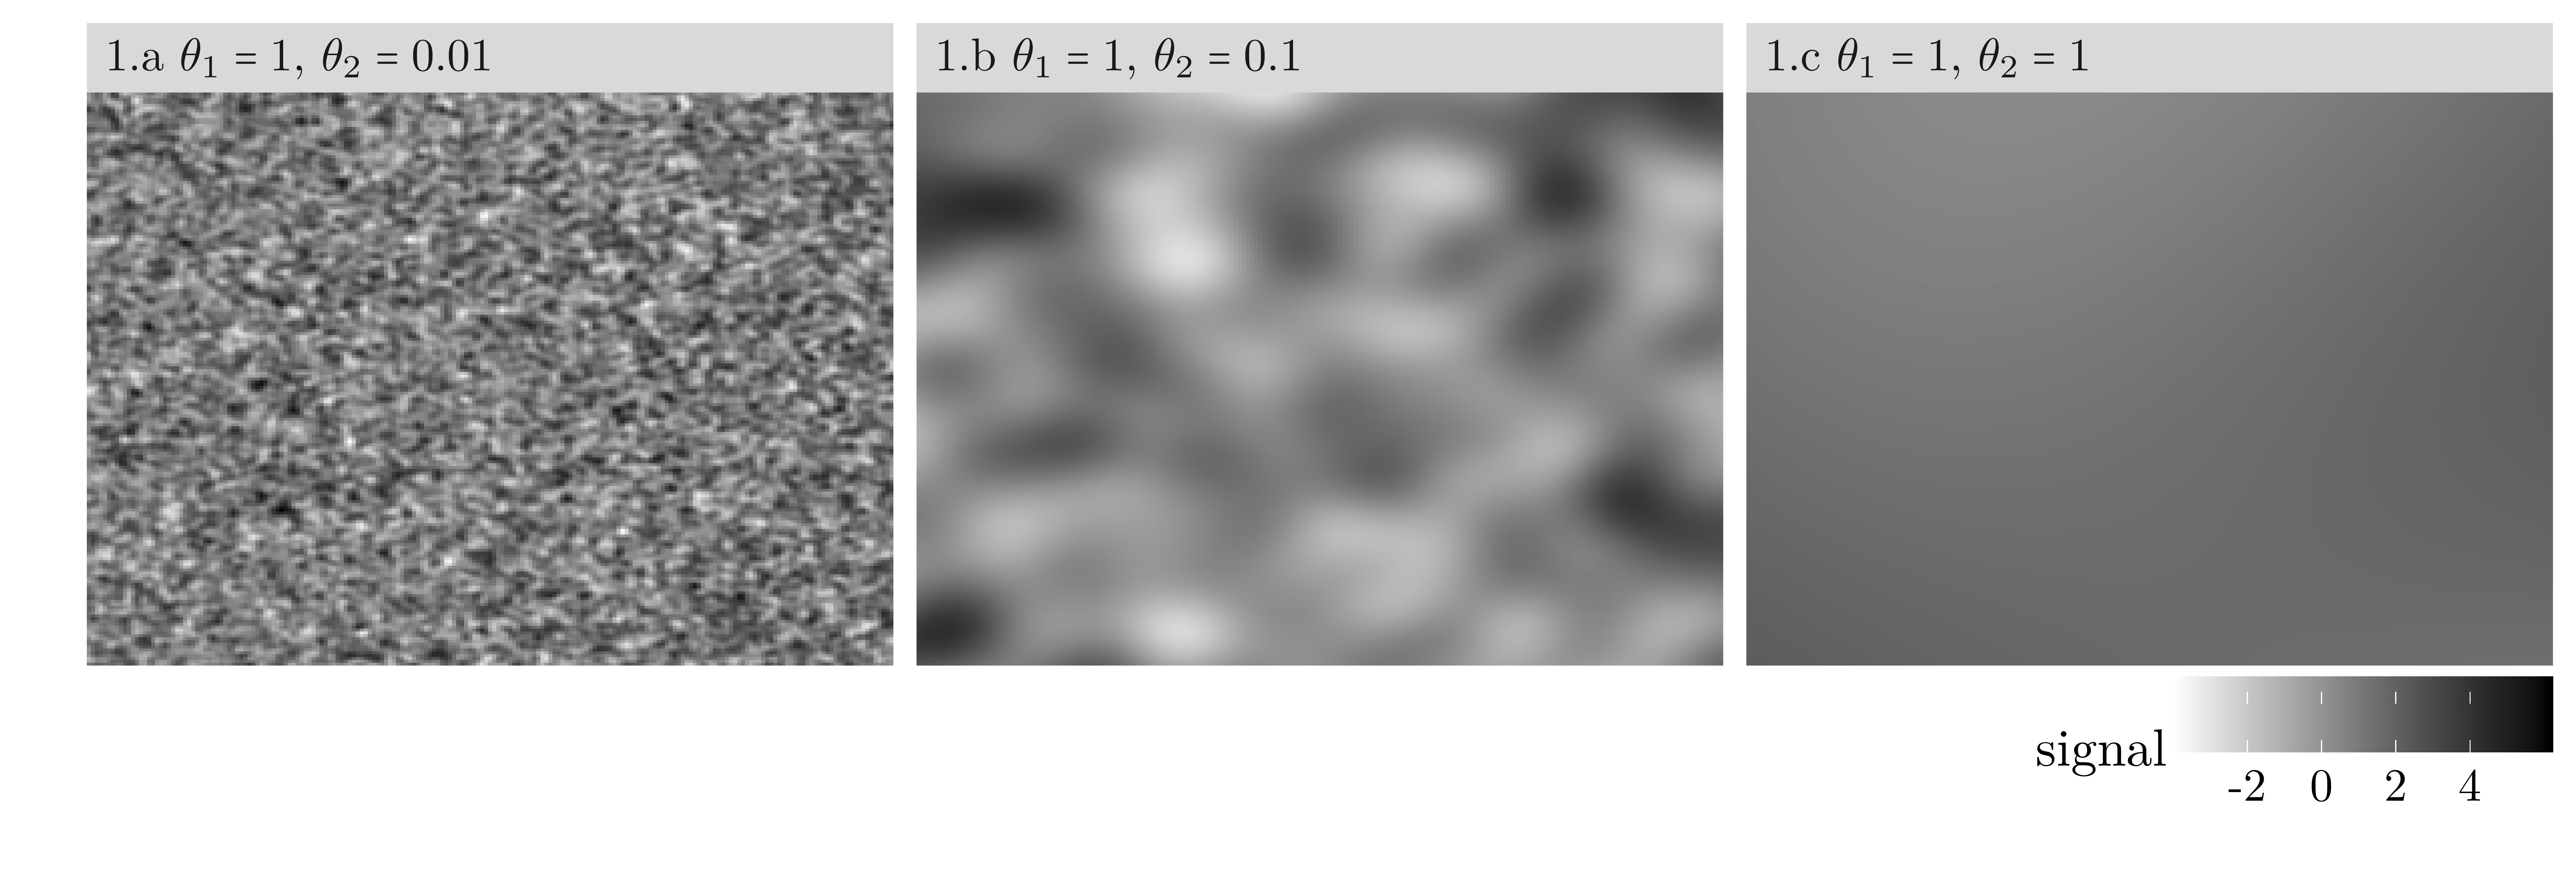
\includegraphics{fig/figure2.png}

%\end{mdframed}

\end{figure}



\begin{figure}[ht]
%\begin{mdframed}
\caption{Joint and marginal densities of $\desvar$ and $\signal$.  Each sub-figure contains the scatter plot of  $\left\{\left(\desvar(\position),\signal(\position)\right):\position\in\mathrm{Grid}\right\}$, where $\mathrm{Grid}$ is a regularly spaced grid of $\Pop$. The values of $(\paramnuisance_0, \paramnuisance_1 ,\paramnuisance_2)$ for each Sub-figure are: 3.a: $(\log(10),0,0)$, 3.b:$(\log(10)-0.125,0,0.5)$, 3.c: $(\log(10)-0.125,0.4,0.3)$. The vertical axis corresponds to $\signal$, the vertical to $\desvar$. The marginal plots correspond to the density of $\desvar$ (right margin) and to the densities of $\signal$ (bottom margins).}\label{fig:jointmarginaldensitiesYZ}
\includegraphics{fig/figure3.png}
%\end{mdframed}
\end{figure}
\end{example}

%$(\Sample[\ell],\Signal[\Sample[\ell]])_{\ell\in\{1,\ldots,\Sampleindex}$
%Observations $(\Sample,\Signal[\Sample])=(\Sample[\ell],\Signal[\Sample[\ell]])_{\ell=1,\ldots,n}$ can be seen as a point process in $\Pop\times\SignalSpace$ and its intensity is defined as the Radon Nikodym derivative of $\Intensity_S$ with respect to the measure $\dominantU\otimes\dominantY$.

\subsection{Probability density function of the sample}

The conditional distributions of the sample and of subsamples can be derived from  the conditional distribution of the design:

\begin{eqnarray}
\density_{\Sample\mid W}(\position\mid\mathbf{w})&=&
\int \left(\derive P^{\Sample\mid \Design,W}/\derive\dominantUbar \right)(\position\mid \design,\mathbf{w})\derive P^{\Design\mid W}(\design\mid\mathbf{w})
\end{eqnarray}

In particular when $W$ is a function of $\Signal$ and $\Desvar$, assumption \eqref{eq:SconditionalonDindependentonYZ} implies that the probability to select the sample $\position$ conditionally on $W=\mathbf{w}$ is the 
probability to select the sample $\position$ given the design, averaged on all possible designs conditionally on  $W=\mathbf{w}$:
\begin{eqnarray}
\density_{\Sample\mid W}(\position\mid\mathbf{w})&=&
\int \left(\derive \design/\derive\dominantUbar \right)(\position)~\derive P^{\Design\mid W}(\design\mid\mathbf{w}).
\end{eqnarray}

\begin{example}[ Example \ref{example:2.2} continued: Sample density for $\Sample\sim \mathrm{Ppp}(\Desvar)$ and $\Sample\sim \mathrm{bpp}(\Desvar,n)$]
\label{example:2.3}
 For $\position\in\Pop^{\{1,\ldots,\samplesize\}}$, when $\Sample\sim \mathrm{Ppp}(\Desvar)$,
\begin{equation}\density_{\Sample\mid W}(\position|\mathbf{w})=
\int\exp\left(-(\desvar.\dominantU)(\Pop)\right)(\samplesize!)^{-1}\left(\prod_{\ell=1}^\samplesize \desvar(\position(\ell))\right)\derive
P^{\Desvar\mid W}(\desvar\mid \mathbf{w}).\label{eq:oijoijejods}
\end{equation}
When $\Sample\sim \mathrm{bpp}(\Desvar,\samplesize)$,
\begin{equation}
\density_{\Sample\mid W}(\position|\mathbf{w})=
\int\left((\desvar.\dominantU)(\Pop)\right)^{-\samplesize}\left(\prod_{\ell=1}^\samplesize \desvar(\position(\ell))\right)\derive
P^{\Desvar\mid W}(\desvar\mid \mathbf{w}).\label{eq:oijerogiql}
\end{equation}
\end{example}




\subsection{Probability density function of a subsample}

Theoretical developments in Section \ref{sec:sampledistribution} require to express the density function of a random size or fixed size subsample of a random or fixed size sample.

For a fixed set $\Sampleindex$, the density 
$\density_{\Sample_\Sampleindex\mid W}(\position\mid\mathbf{w})$
can be derived from $\density_{\Sample\mid W}$ via:
\begin{eqnarray}
\density_{\Sample_\Sampleindex\mid W}(\position\mid\mathbf{w})&=&
\int \density_{\Sample\mid W}(\position'\mid \mathbf{w})~\mathds{1}(\position'_\Sampleindex==\position)~\derive\dominantUbar(\position'),
\end{eqnarray}
where $\mathds{1}(\position'_\Sampleindex==\position)=0$ when $\position'_\Sampleindex!=\position$, $1$ otherwise.  
More generally, for a random set $\Sampleindex$ the density 
$\density_{\Sample\mid W}(\position\mid\mathbf{w})$
can be derived from $\density_{\Sample_\Sampleindex\mid W}$ via:
\begin{eqnarray}
\density_{\Sample_\Sampleindex\mid W}(\position\mid\mathbf{w})&=&
\int\left(\int \density_{\Sample\mid W}(\position'\mid \mathbf{w})~\mathds{1}(\position'_\Sampleindex==\position)~\derive\dominantUbar(\position')\right)\derive P^{K\mid W=\mathbf{w}}.
\end{eqnarray}

\begin{remark}\label{remark:K1subsetK2}
For  two fixed size sets  $\Sampleindex_1, \Sampleindex_2$ fixed such that 
$\Sampleindex_1\subset \Sampleindex_2$, the equation 
\begin{equation}\label{eq:iugheirguhei}\density_{\Sample_{\Sampleindex_1}}(\position\mid \mathbf{w})=\int \density_{\Sample_{\Sampleindex_2}}(\position'\mid \mathbf{w})\mathds{1}(\position'_{\Sampleindex_1}=\position)\derive \dominantU^{\otimes K_2}(\position')
\end{equation}
is not necessarily true. 
For example, when $S\sim \mathrm{Ppp}(\Desvar)$, 
$\Sampleindex_1=\{1\}$, $\Sampleindex_2=\{1,2\}$,
for $\position \in \Pop^{\{1\}}$, 
$\density_{\Sample_{\{1\}}}(\position)=\density_{\Sample}(\position)+\int \density_{\Sample_{\Sampleindex_2}}(\position'\mid \mathbf{w})\mathds{1}(\position'_{\Sampleindex_1}=\position)\derive \dominantU^{\otimes K_2}(\position')$.
A sufficient condition for the equation \eqref{eq:iugheirguhei} would be that $\Samplesize$ is not random.
\end{remark}

Let $\Sampleindex$ be  a finite subset of $\mathbb{N}\setminus\{0\}$. Let   $\Sampleindex'$ be an element of $\{\{\ell\in \Sampleindex:\ell\leq\samplesize\}:\samplesize\in\mathbb{N}\}$, and let  $\position\in\Pop^{\Sampleindex'}$. Let $W$ be a function of $\Desvar$, $\Signal$.
In the following we derive the density of $\Sample_\Sampleindex$ conditionally on $W=\mathbf{w}$.
For $\position=\mathbf{0}$,
\begin{equation}\density_{\Sample_K\mid W}(\mathbf{0}\mid\mathbf{w})=\left|\begin{array}{ll}1&\text{if }\Sampleindex=\emptyset,\\
P(\Samplesize<\min(K)\mid W=\mathbf{w})&\text{ otherwise.}
\end{array}\right.\end{equation}
For $\position\neq\mathbf{0}$,
\begin{equation}\label{eq:iduhifduewer}
\density_{\Sample_K\mid W}(\position\mid\mathbf{w})=
\int \density_{\Sample_K\mid \Desvar}(\position\mid\desvar) \derive P^{\Desvar\mid W}(\desvar\mid\mathbf{w}).
\end{equation}
\begin{example}[Example \ref{example:2.3} continued: Probability density function of a subsample for $\Sample\sim \mathrm{Ppp}(\Desvar)$ and $\Sample\sim \mathrm{bpp}(\Desvar,\samplesize)$ .]
\label{example:2.4}

Let $\Sampleindex$ be  a non random  finite subset of $\mathbb{N}\setminus\{0\}$

When $\Sample\sim \mathrm{Ppp}(\Desvar)$,
\begin{equation}\label{eq:sgiushdiuh}
\density_{\Sample_K\mid \Desvar}(\position\mid\mathbf{\desvar})=
\left(\sum_{\substack{\samplesize\in\mathbb{N}:\\\{\ell\in\Sampleindex:\ell\leq\samplesize\}=\Sampleindex'}}\!\!\!\!\!\!\!\! P(\Samplesize=\samplesize\mid\Desvar=\desvar)\right)\prod_{\ell\in\Sampleindex'}\frac{\desvar(\position(\ell))}{(\desvar.\dominantU)(\Pop)}.
\end{equation}


and when $\Sample\sim \mathrm{bpp}(\Desvar,\samplesize)$,
\begin{equation}\label{eq:sgiushdiuh2}
\density_{\Sample_{\Sampleindex}\mid \Desvar}(\position|\desvar)=\left|\begin{array}{ll}
\prod_{\ell\in\Sampleindex'} \left(\left((\desvar.\dominantU)(\Pop)\right)^{-1}\left(\desvar(\position(\ell))\right)\right)&\text{if }\Sampleindex'=\{1,\ldots,\samplesize\}\cap\Sampleindex\\
0&\text{otherwise.}
\end{array}\right.\end{equation}






\end{example}

Note that the distribution of the sample unconditionally on the design or the design variable can be obtained via: 
$\density_{\Sample}(\position)=\int \density_{\Sample\mid\Desvar}(\position)\derive P^\Desvar$.
Contrary to the particular case of population index exchangeability and sample index exchangeability, the sample index exchangeability \eqref{assumption:designindexexchangeability} condition alone does not ensure that conditionally on the sample size, $\Samplesize=\samplesize$, the distribution of the sample  $P^{\Sample\mid\Samplesize=\samplesize}$ is the uniform distribution on $\Pop^{\{1,\ldots,\samplesize\}}$. 
For example, $f_{\Sample_{\{1\}}}$ can be uniform, but $f_{\Sample_{\{1,2\}}}$ not.
